\documentclass[1p]{elsarticle_modified}
%\bibliographystyle{elsarticle-num}

%\usepackage[colorlinks]{hyperref}
%\usepackage{abbrmath_seonhwa} %\Abb, \Ascr, \Acal ,\Abf, \Afrak
\usepackage{amsfonts}
\usepackage{amssymb}
\usepackage{amsmath}
\usepackage{amsthm}
\usepackage{scalefnt}
\usepackage{amsbsy}
\usepackage{kotex}
\usepackage{caption}
\usepackage{subfig}
\usepackage{color}
\usepackage{graphicx}
\usepackage{xcolor} %% white, black, red, green, blue, cyan, magenta, yellow
\usepackage{float}
\usepackage{setspace}
\usepackage{hyperref}

\usepackage{tikz}
\usetikzlibrary{arrows}

\usepackage{multirow}
\usepackage{array} % fixed length table
\usepackage{hhline}

%%%%%%%%%%%%%%%%%%%%%
\makeatletter
\renewcommand*\env@matrix[1][\arraystretch]{%
	\edef\arraystretch{#1}%
	\hskip -\arraycolsep
	\let\@ifnextchar\new@ifnextchar
	\array{*\c@MaxMatrixCols c}}
\makeatother %https://tex.stackexchange.com/questions/14071/how-can-i-increase-the-line-spacing-in-a-matrix
%%%%%%%%%%%%%%%

\usepackage[normalem]{ulem}

\newcommand{\msout}[1]{\ifmmode\text{\sout{\ensuremath{#1}}}\else\sout{#1}\fi}
%SOURCE: \msout is \stkout macro in https://tex.stackexchange.com/questions/20609/strikeout-in-math-mode

\newcommand{\cancel}[1]{
	\ifmmode
	{\color{red}\msout{#1}}
	\else
	{\color{red}\sout{#1}}
	\fi
}

\newcommand{\add}[1]{
	{\color{blue}\uwave{#1}}
}

\newcommand{\replace}[2]{
	\ifmmode
	{\color{red}\msout{#1}}{\color{blue}\uwave{#2}}
	\else
	{\color{red}\sout{#1}}{\color{blue}\uwave{#2}}
	\fi
}

\newcommand{\Sol}{\mathcal{S}} %segment
\newcommand{\D}{D} %diagram
\newcommand{\A}{\mathcal{A}} %arc


%%%%%%%%%%%%%%%%%%%%%%%%%%%%%5 test

\def\sl{\operatorname{\textup{SL}}(2,\Cbb)}
\def\psl{\operatorname{\textup{PSL}}(2,\Cbb)}
\def\quan{\mkern 1mu \triangleright \mkern 1mu}

\theoremstyle{definition}
\newtheorem{thm}{Theorem}[section]
\newtheorem{prop}[thm]{Proposition}
\newtheorem{lem}[thm]{Lemma}
\newtheorem{ques}[thm]{Question}
\newtheorem{cor}[thm]{Corollary}
\newtheorem{defn}[thm]{Definition}
\newtheorem{exam}[thm]{Example}
\newtheorem{rmk}[thm]{Remark}
\newtheorem{alg}[thm]{Algorithm}

\newcommand{\I}{\sqrt{-1}}
\begin{document}

%\begin{frontmatter}
%
%\title{Boundary parabolic representations of knots up to 8 crossings}
%
%%% Group authors per affiliation:
%\author{Yunhi Cho} 
%\address{Department of Mathematics, University of Seoul, Seoul, Korea}
%\ead{yhcho@uos.ac.kr}
%
%
%\author{Seonhwa Kim} %\fnref{s_kim}}
%\address{Center for Geometry and Physics, Institute for Basic Science, Pohang, 37673, Korea}
%\ead{ryeona17@ibs.re.kr}
%
%\author{Hyuk Kim}
%\address{Department of Mathematical Sciences, Seoul National University, Seoul 08826, Korea}
%\ead{hyukkim@snu.ac.kr}
%
%\author{Seokbeom Yoon}
%\address{Department of Mathematical Sciences, Seoul National University, Seoul, 08826,  Korea}
%\ead{sbyoon15@snu.ac.kr}
%
%\begin{abstract}
%We find all boundary parabolic representation of knots up to 8 crossings.
%
%\end{abstract}
%\begin{keyword}
%    \MSC[2010] 57M25 
%\end{keyword}
%
%\end{frontmatter}

%\linenumbers
%\tableofcontents
%
\newcommand\colored[1]{\textcolor{white}{\rule[-0.35ex]{0.8em}{1.4ex}}\kern-0.8em\color{red} #1}%
%\newcommand\colored[1]{\textcolor{white}{ #1}\kern-2.17ex	\textcolor{white}{ #1}\kern-1.81ex	\textcolor{white}{ #1}\kern-2.15ex\color{red}#1	}

{\Large $\underline{12a_{1096}~(K12a_{1096})}$}

\setlength{\tabcolsep}{10pt}
\renewcommand{\arraystretch}{1.6}
\vspace{1cm}\begin{tabular}{m{100pt}>{\centering\arraybackslash}m{274pt}}
\multirow{5}{120pt}{
	\centering
	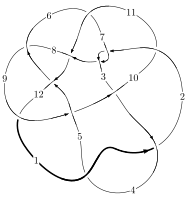
\includegraphics[width=112pt]{../../../GIT/diagram.site/Diagrams/png/1897_12a_1096.png}\\
\ \ \ A knot diagram\footnotemark}&
\allowdisplaybreaks
\textbf{Linearized knot diagam} \\
\cline{2-2}
 &
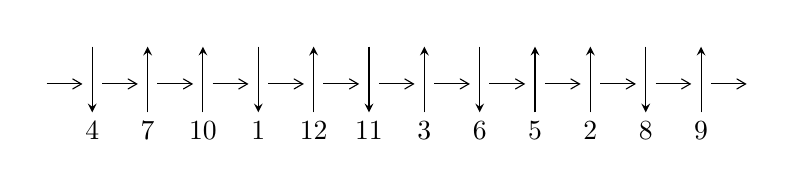
\begin{tikzpicture}[x=20pt, y=17pt]
	% nodes
	\node (C0) at (0, 0) {};
	\node (C1) at (1, 0) {};
	\node (C1U) at (1, +1) {};
	\node (C1D) at (1, -1) {4};

	\node (C2) at (2, 0) {};
	\node (C2U) at (2, +1) {};
	\node (C2D) at (2, -1) {7};

	\node (C3) at (3, 0) {};
	\node (C3U) at (3, +1) {};
	\node (C3D) at (3, -1) {10};

	\node (C4) at (4, 0) {};
	\node (C4U) at (4, +1) {};
	\node (C4D) at (4, -1) {1};

	\node (C5) at (5, 0) {};
	\node (C5U) at (5, +1) {};
	\node (C5D) at (5, -1) {12};

	\node (C6) at (6, 0) {};
	\node (C6U) at (6, +1) {};
	\node (C6D) at (6, -1) {11};

	\node (C7) at (7, 0) {};
	\node (C7U) at (7, +1) {};
	\node (C7D) at (7, -1) {3};

	\node (C8) at (8, 0) {};
	\node (C8U) at (8, +1) {};
	\node (C8D) at (8, -1) {6};

	\node (C9) at (9, 0) {};
	\node (C9U) at (9, +1) {};
	\node (C9D) at (9, -1) {5};

	\node (C10) at (10, 0) {};
	\node (C10U) at (10, +1) {};
	\node (C10D) at (10, -1) {2};

	\node (C11) at (11, 0) {};
	\node (C11U) at (11, +1) {};
	\node (C11D) at (11, -1) {8};

	\node (C12) at (12, 0) {};
	\node (C12U) at (12, +1) {};
	\node (C12D) at (12, -1) {9};
	\node (C13) at (13, 0) {};

	% arrows
	\draw[->,>={angle 60}]
	(C0) edge (C1) (C1) edge (C2) (C2) edge (C3) (C3) edge (C4) (C4) edge (C5) (C5) edge (C6) (C6) edge (C7) (C7) edge (C8) (C8) edge (C9) (C9) edge (C10) (C10) edge (C11) (C11) edge (C12) (C12) edge (C13) ;	\draw[->,>=stealth]
	(C1U) edge (C1D) (C2D) edge (C2U) (C3D) edge (C3U) (C4U) edge (C4D) (C5D) edge (C5U) (C6U) edge (C6D) (C7D) edge (C7U) (C8U) edge (C8D) (C9D) edge (C9U) (C10D) edge (C10U) (C11U) edge (C11D) (C12D) edge (C12U) ;
	\end{tikzpicture} \\
\hhline{~~} \\& 
\textbf{Solving Sequence} \\ \cline{2-2} 
 &
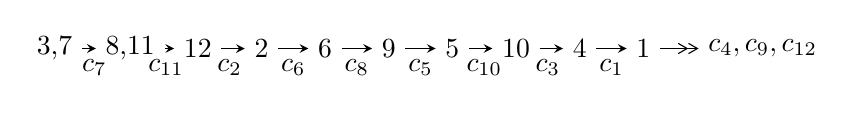
\begin{tikzpicture}[x=23pt, y=7pt]
	% node
	\node (A0) at (-1/8, 0) {3,7};
	\node (A1) at (17/16, 0) {8,11};
	\node (A2) at (17/8, 0) {12};
	\node (A3) at (25/8, 0) {2};
	\node (A4) at (33/8, 0) {6};
	\node (A5) at (41/8, 0) {9};
	\node (A6) at (49/8, 0) {5};
	\node (A7) at (57/8, 0) {10};
	\node (A8) at (65/8, 0) {4};
	\node (A9) at (73/8, 0) {1};
	\node (C1) at (1/2, -1) {$c_{7}$};
	\node (C2) at (13/8, -1) {$c_{11}$};
	\node (C3) at (21/8, -1) {$c_{2}$};
	\node (C4) at (29/8, -1) {$c_{6}$};
	\node (C5) at (37/8, -1) {$c_{8}$};
	\node (C6) at (45/8, -1) {$c_{5}$};
	\node (C7) at (53/8, -1) {$c_{10}$};
	\node (C8) at (61/8, -1) {$c_{3}$};
	\node (C9) at (69/8, -1) {$c_{1}$};
	\node (A10) at (11, 0) {$c_{4},c_{9},c_{12}$};

	% edge
	\draw[->,>=stealth]	
	(A0) edge (A1) (A1) edge (A2) (A2) edge (A3) (A3) edge (A4) (A4) edge (A5) (A5) edge (A6) (A6) edge (A7) (A7) edge (A8) (A8) edge (A9) ;
	\draw[->>,>={angle 60}]	
	(A9) edge (A10);
\end{tikzpicture} \\ 

\end{tabular} \\

\footnotetext{
The image of knot diagram is generated by the software ``\textbf{Draw programme}" developed by Andrew Bartholomew(\url{http://www.layer8.co.uk/maths/draw/index.htm\#Running-draw}), where we modified some parts for our purpose(\url{https://github.com/CATsTAILs/LinksPainter}).
}\phantom \\ \newline 
\centering \textbf{Ideals for irreducible components\footnotemark of $X_{\text{par}}$} 
 
\begin{align*}
I^u_{1}&=\langle 
1.80914\times10^{961} u^{171}+1.79843\times10^{961} u^{170}+\cdots+7.62520\times10^{962} b-2.39787\times10^{966},\\
\phantom{I^u_{1}}&\phantom{= \langle  }-2.31980\times10^{966} u^{171}-1.92030\times10^{966} u^{170}+\cdots+6.27020\times10^{966} a+1.72930\times10^{971},\\
\phantom{I^u_{1}}&\phantom{= \langle  }u^{172}-50 u^{170}+\cdots+24120 u+74007\rangle \\
I^u_{2}&=\langle 
-5.15815\times10^{26} u^{36}+2.11275\times10^{26} u^{35}+\cdots+4.28196\times10^{25} b-7.24553\times10^{26},\\
\phantom{I^u_{2}}&\phantom{= \langle  }-1.49365\times10^{27} u^{36}+8.00234\times10^{26} u^{35}+\cdots+4.28196\times10^{25} a-3.46005\times10^{27},\;u^{37}- u^{36}+\cdots+4 u-1\rangle \\
\\
\end{align*}
\raggedright * 2 irreducible components of $\dim_{\mathbb{C}}=0$, with total 209 representations.\\
\footnotetext{All coefficients of polynomials are rational numbers. But the coefficients are sometimes approximated in decimal forms when there is not enough margin.}
\newpage
\renewcommand{\arraystretch}{1}
\centering \section*{I. $I^u_{1}= \langle 1.81\times10^{961} u^{171}+1.80\times10^{961} u^{170}+\cdots+7.63\times10^{962} b-2.40\times10^{966},\;-2.32\times10^{966} u^{171}-1.92\times10^{966} u^{170}+\cdots+6.27\times10^{966} a+1.73\times10^{971},\;u^{172}-50 u^{170}+\cdots+24120 u+74007 \rangle$}
\flushleft \textbf{(i) Arc colorings}\\
\begin{tabular}{m{7pt} m{180pt} m{7pt} m{180pt} }
\flushright $a_{3}=$&$\begin{pmatrix}0\\u\end{pmatrix}$ \\
\flushright $a_{7}=$&$\begin{pmatrix}1\\0\end{pmatrix}$ \\
\flushright $a_{8}=$&$\begin{pmatrix}1\\- u^2\end{pmatrix}$ \\
\flushright $a_{11}=$&$\begin{pmatrix}0.369973 u^{171}+0.306258 u^{170}+\cdots-41770.3 u-27579.6\\-0.0237258 u^{171}-0.0235853 u^{170}+\cdots+2274.90 u+3144.67\end{pmatrix}$ \\
\flushright $a_{12}=$&$\begin{pmatrix}0.0801750 u^{171}+0.0701081 u^{170}+\cdots-9277.69 u-8058.99\\0.214417 u^{171}+0.185788 u^{170}+\cdots-24868.1 u-14332.1\end{pmatrix}$ \\
\flushright $a_{2}=$&$\begin{pmatrix}- u\\u\end{pmatrix}$ \\
\flushright $a_{6}=$&$\begin{pmatrix}-0.116749 u^{171}-0.0884275 u^{170}+\cdots+10576.9 u+6108.56\\0.00487777 u^{171}-0.00935276 u^{170}+\cdots+2795.37 u+3971.83\end{pmatrix}$ \\
\flushright $a_{9}=$&$\begin{pmatrix}-0.206611 u^{171}-0.296700 u^{170}+\cdots+15684.9 u+19751.0\\0.218769 u^{171}+0.274949 u^{170}+\cdots-19308.1 u-19958.5\end{pmatrix}$ \\
\flushright $a_{5}=$&$\begin{pmatrix}0.0142311 u^{171}+0.0188741 u^{170}+\cdots-3030.69 u-2555.15\\0.368988 u^{171}+0.357759 u^{170}+\cdots-39066.5 u-28688.6\end{pmatrix}$ \\
\flushright $a_{10}=$&$\begin{pmatrix}0.0859178 u^{171}+0.0620963 u^{170}+\cdots-9327.55 u-6659.80\\0.260329 u^{171}+0.220577 u^{170}+\cdots-30167.9 u-17775.1\end{pmatrix}$ \\
\flushright $a_{4}=$&$\begin{pmatrix}-0.0430210 u^{171}-0.0850699 u^{170}+\cdots+2192.62 u+4621.27\\-0.0662657 u^{171}-0.0164058 u^{170}+\cdots+10891.5 u+5135.15\end{pmatrix}$ \\
\flushright $a_{1}=$&$\begin{pmatrix}0.143934 u^{171}+0.138978 u^{170}+\cdots-13771.4 u-11391.8\\0.0192585 u^{171}+0.00519459 u^{170}+\cdots-2742.25 u+179.012\end{pmatrix}$\\&\end{tabular}
\flushleft \textbf{(ii) Obstruction class $= -1$}\\~\\
\flushleft \textbf{(iii) Cusp Shapes $= 0.0528030 u^{171}+0.682581 u^{170}+\cdots-15889.4 u-58849.8$}\\~\\
\newpage\renewcommand{\arraystretch}{1}
\flushleft \textbf{(iv) u-Polynomials at the component}\newline \\
\begin{tabular}{m{50pt}|m{274pt}}
Crossings & \hspace{64pt}u-Polynomials at each crossing \\
\hline $$\begin{aligned}c_{1},c_{4}\end{aligned}$$&$\begin{aligned}
&u^{172}-9 u^{171}+\cdots-100 u+1
\end{aligned}$\\
\hline $$\begin{aligned}c_{2},c_{7}\end{aligned}$$&$\begin{aligned}
&u^{172}-50 u^{170}+\cdots-24120 u+74007
\end{aligned}$\\
\hline $$\begin{aligned}c_{3}\end{aligned}$$&$\begin{aligned}
&u^{172}+7 u^{171}+\cdots-919920 u-65828
\end{aligned}$\\
\hline $$\begin{aligned}c_{5}\end{aligned}$$&$\begin{aligned}
&u^{172}-7 u^{171}+\cdots+10616 u-167
\end{aligned}$\\
\hline $$\begin{aligned}c_{6}\end{aligned}$$&$\begin{aligned}
&u^{172}-7 u^{171}+\cdots-87748249 u-53910283
\end{aligned}$\\
\hline $$\begin{aligned}c_{8}\end{aligned}$$&$\begin{aligned}
&u^{172}-19 u^{171}+\cdots+285466 u-10697
\end{aligned}$\\
\hline $$\begin{aligned}c_{9}\end{aligned}$$&$\begin{aligned}
&u^{172}-11 u^{171}+\cdots-160 u-7
\end{aligned}$\\
\hline $$\begin{aligned}c_{10}\end{aligned}$$&$\begin{aligned}
&u^{172}-7 u^{171}+\cdots+503175069 u-16162283
\end{aligned}$\\
\hline $$\begin{aligned}c_{11}\end{aligned}$$&$\begin{aligned}
&u^{172}-4 u^{171}+\cdots+77660 u-9916
\end{aligned}$\\
\hline $$\begin{aligned}c_{12}\end{aligned}$$&$\begin{aligned}
&u^{172}-18 u^{170}+\cdots+1012767 u+106551
\end{aligned}$\\
\hline
\end{tabular}\\~\\
\newpage\renewcommand{\arraystretch}{1}
\flushleft \textbf{(v) Riley Polynomials at the component}\newline \\
\begin{tabular}{m{50pt}|m{274pt}}
Crossings & \hspace{64pt}Riley Polynomials at each crossing \\
\hline $$\begin{aligned}c_{1},c_{4}\end{aligned}$$&$\begin{aligned}
&y^{172}+127 y^{171}+\cdots-3840 y+1
\end{aligned}$\\
\hline $$\begin{aligned}c_{2},c_{7}\end{aligned}$$&$\begin{aligned}
&y^{172}-100 y^{171}+\cdots-159358760424 y+5477036049
\end{aligned}$\\
\hline $$\begin{aligned}c_{3}\end{aligned}$$&$\begin{aligned}
&y^{172}-23 y^{171}+\cdots+56985557264 y+4333325584
\end{aligned}$\\
\hline $$\begin{aligned}c_{5}\end{aligned}$$&$\begin{aligned}
&y^{172}+9 y^{171}+\cdots-70838234 y+27889
\end{aligned}$\\
\hline $$\begin{aligned}c_{6}\end{aligned}$$&$\begin{aligned}
&y^{172}+47 y^{171}+\cdots+2003456514376098053 y+2906318613140089
\end{aligned}$\\
\hline $$\begin{aligned}c_{8}\end{aligned}$$&$\begin{aligned}
&y^{172}+37 y^{171}+\cdots+5944665142 y+114425809
\end{aligned}$\\
\hline $$\begin{aligned}c_{9}\end{aligned}$$&$\begin{aligned}
&y^{172}-21 y^{171}+\cdots-3648 y+49
\end{aligned}$\\
\hline $$\begin{aligned}c_{10}\end{aligned}$$&$\begin{aligned}
&y^{172}-53 y^{171}+\cdots-88286474877028847 y+261219391772089
\end{aligned}$\\
\hline $$\begin{aligned}c_{11}\end{aligned}$$&$\begin{aligned}
&y^{172}-12 y^{171}+\cdots-3415353792 y+98327056
\end{aligned}$\\
\hline $$\begin{aligned}c_{12}\end{aligned}$$&$\begin{aligned}
&y^{172}-36 y^{171}+\cdots-1103499684081 y+11353115601
\end{aligned}$\\
\hline
\end{tabular}\\~\\
\newpage\flushleft \textbf{(vi) Complex Volumes and Cusp Shapes}
$$\begin{array}{c|c|c}  
\text{Solutions to }I^u_{1}& \I (\text{vol} + \sqrt{-1}CS) & \text{Cusp shape}\\
 \hline 
\begin{aligned}
u &= -0.964700 + 0.292936 I \\
a &= \phantom{-}0.975586 + 0.348053 I \\
b &= -2.03350 + 0.07508 I\end{aligned}
 & \phantom{-}2.75116 - 11.23960 I & \phantom{-0.000000 } 0 \\ \hline\begin{aligned}
u &= -0.964700 - 0.292936 I \\
a &= \phantom{-}0.975586 - 0.348053 I \\
b &= -2.03350 - 0.07508 I\end{aligned}
 & \phantom{-}2.75116 + 11.23960 I & \phantom{-0.000000 } 0 \\ \hline\begin{aligned}
u &= -0.963724 + 0.227184 I \\
a &= -0.72179 - 2.61850 I \\
b &= \phantom{-}0.461935 + 0.786477 I\end{aligned}
 & -0.66871 - 6.23689 I & \phantom{-0.000000 } 0 \\ \hline\begin{aligned}
u &= -0.963724 - 0.227184 I \\
a &= -0.72179 + 2.61850 I \\
b &= \phantom{-}0.461935 - 0.786477 I\end{aligned}
 & -0.66871 + 6.23689 I & \phantom{-0.000000 } 0 \\ \hline\begin{aligned}
u &= -0.954904 + 0.236922 I \\
a &= \phantom{-}0.46983 + 2.19175 I \\
b &= -0.072423 - 1.127430 I\end{aligned}
 & -0.89758 - 1.41134 I & \phantom{-0.000000 } 0 \\ \hline\begin{aligned}
u &= -0.954904 - 0.236922 I \\
a &= \phantom{-}0.46983 - 2.19175 I \\
b &= -0.072423 + 1.127430 I\end{aligned}
 & -0.89758 + 1.41134 I & \phantom{-0.000000 } 0 \\ \hline\begin{aligned}
u &= \phantom{-}0.978570 + 0.079158 I \\
a &= -1.22031 + 1.55246 I \\
b &= -0.398043 - 0.997722 I\end{aligned}
 & \phantom{-}6.95288 + 0.33712 I & \phantom{-0.000000 } 0 \\ \hline\begin{aligned}
u &= \phantom{-}0.978570 - 0.079158 I \\
a &= -1.22031 - 1.55246 I \\
b &= -0.398043 + 0.997722 I\end{aligned}
 & \phantom{-}6.95288 - 0.33712 I & \phantom{-0.000000 } 0 \\ \hline\begin{aligned}
u &= \phantom{-}0.817320 + 0.541096 I \\
a &= -0.002993 - 1.051400 I \\
b &= \phantom{-}0.338375 + 0.341192 I\end{aligned}
 & -3.13276 + 2.18455 I & \phantom{-0.000000 } 0 \\ \hline\begin{aligned}
u &= \phantom{-}0.817320 - 0.541096 I \\
a &= -0.002993 + 1.051400 I \\
b &= \phantom{-}0.338375 - 0.341192 I\end{aligned}
 & -3.13276 - 2.18455 I & \phantom{-0.000000 } 0\\
 \hline 
 \end{array}$$\newpage$$\begin{array}{c|c|c}  
\text{Solutions to }I^u_{1}& \I (\text{vol} + \sqrt{-1}CS) & \text{Cusp shape}\\
 \hline 
\begin{aligned}
u &= -0.920977 + 0.328617 I \\
a &= \phantom{-}0.24862 - 2.48894 I \\
b &= \phantom{-}1.17628 + 1.16599 I\end{aligned}
 & \phantom{-}3.09198 - 2.40359 I & \phantom{-0.000000 } 0 \\ \hline\begin{aligned}
u &= -0.920977 - 0.328617 I \\
a &= \phantom{-}0.24862 + 2.48894 I \\
b &= \phantom{-}1.17628 - 1.16599 I\end{aligned}
 & \phantom{-}3.09198 + 2.40359 I & \phantom{-0.000000 } 0 \\ \hline\begin{aligned}
u &= -0.875584 + 0.426153 I \\
a &= \phantom{-}0.35185 + 2.28506 I \\
b &= -1.77192 - 0.47812 I\end{aligned}
 & \phantom{-}3.21409 - 1.23569 I & \phantom{-0.000000 } 0 \\ \hline\begin{aligned}
u &= -0.875584 - 0.426153 I \\
a &= \phantom{-}0.35185 - 2.28506 I \\
b &= -1.77192 + 0.47812 I\end{aligned}
 & \phantom{-}3.21409 + 1.23569 I & \phantom{-0.000000 } 0 \\ \hline\begin{aligned}
u &= \phantom{-}1.022970 + 0.082774 I \\
a &= \phantom{-}2.55671 - 4.44659 I \\
b &= -2.44884 + 4.07782 I\end{aligned}
 & \phantom{-}5.06247 + 0.18677 I & \phantom{-0.000000 } 0 \\ \hline\begin{aligned}
u &= \phantom{-}1.022970 - 0.082774 I \\
a &= \phantom{-}2.55671 + 4.44659 I \\
b &= -2.44884 - 4.07782 I\end{aligned}
 & \phantom{-}5.06247 - 0.18677 I & \phantom{-0.000000 } 0 \\ \hline\begin{aligned}
u &= -0.862990 + 0.421595 I \\
a &= \phantom{-}0.02548 - 2.91685 I \\
b &= \phantom{-}2.18244 + 1.13167 I\end{aligned}
 & \phantom{-}3.04420 - 2.37891 I & \phantom{-0.000000 } 0 \\ \hline\begin{aligned}
u &= -0.862990 - 0.421595 I \\
a &= \phantom{-}0.02548 + 2.91685 I \\
b &= \phantom{-}2.18244 - 1.13167 I\end{aligned}
 & \phantom{-}3.04420 + 2.37891 I & \phantom{-0.000000 } 0 \\ \hline\begin{aligned}
u &= \phantom{-}0.875550 + 0.392754 I \\
a &= \phantom{-}0.786018 - 0.096425 I \\
b &= -1.51763 - 0.22252 I\end{aligned}
 & -2.17919 + 7.01592 I & \phantom{-0.000000 } 0 \\ \hline\begin{aligned}
u &= \phantom{-}0.875550 - 0.392754 I \\
a &= \phantom{-}0.786018 + 0.096425 I \\
b &= -1.51763 + 0.22252 I\end{aligned}
 & -2.17919 - 7.01592 I & \phantom{-0.000000 } 0\\
 \hline 
 \end{array}$$\newpage$$\begin{array}{c|c|c}  
\text{Solutions to }I^u_{1}& \I (\text{vol} + \sqrt{-1}CS) & \text{Cusp shape}\\
 \hline 
\begin{aligned}
u &= -0.172939 + 0.941887 I \\
a &= -0.064330 - 0.189557 I \\
b &= \phantom{-}0.572184 - 1.130890 I\end{aligned}
 & \phantom{-}5.89144 + 6.63249 I & \phantom{-0.000000 } 0 \\ \hline\begin{aligned}
u &= -0.172939 - 0.941887 I \\
a &= -0.064330 + 0.189557 I \\
b &= \phantom{-}0.572184 + 1.130890 I\end{aligned}
 & \phantom{-}5.89144 - 6.63249 I & \phantom{-0.000000 } 0 \\ \hline\begin{aligned}
u &= -0.107387 + 1.036830 I \\
a &= \phantom{-}0.092726 + 0.492378 I \\
b &= -0.596190 + 0.404651 I\end{aligned}
 & \phantom{-}0.49611 + 6.13968 I & \phantom{-0.000000 } 0 \\ \hline\begin{aligned}
u &= -0.107387 - 1.036830 I \\
a &= \phantom{-}0.092726 - 0.492378 I \\
b &= -0.596190 - 0.404651 I\end{aligned}
 & \phantom{-}0.49611 - 6.13968 I & \phantom{-0.000000 } 0 \\ \hline\begin{aligned}
u &= \phantom{-}0.793137 + 0.533960 I \\
a &= \phantom{-}3.19346 - 0.78504 I \\
b &= -2.04681 - 2.58728 I\end{aligned}
 & \phantom{-}3.49762 + 2.24763 I & \phantom{-0.000000 } 0 \\ \hline\begin{aligned}
u &= \phantom{-}0.793137 - 0.533960 I \\
a &= \phantom{-}3.19346 + 0.78504 I \\
b &= -2.04681 + 2.58728 I\end{aligned}
 & \phantom{-}3.49762 - 2.24763 I & \phantom{-0.000000 } 0 \\ \hline\begin{aligned}
u &= -1.024410 + 0.239856 I \\
a &= -0.625377 + 0.524991 I \\
b &= \phantom{-}1.55133 - 0.60014 I\end{aligned}
 & \phantom{-}1.10082 - 4.32017 I & \phantom{-0.000000 } 0 \\ \hline\begin{aligned}
u &= -1.024410 - 0.239856 I \\
a &= -0.625377 - 0.524991 I \\
b &= \phantom{-}1.55133 + 0.60014 I\end{aligned}
 & \phantom{-}1.10082 + 4.32017 I & \phantom{-0.000000 } 0 \\ \hline\begin{aligned}
u &= \phantom{-}0.989545 + 0.375351 I \\
a &= -0.13531 + 2.44805 I \\
b &= \phantom{-}0.841861 - 0.882838 I\end{aligned}
 & \phantom{-}2.33287 + 11.95800 I & \phantom{-0.000000 } 0 \\ \hline\begin{aligned}
u &= \phantom{-}0.989545 - 0.375351 I \\
a &= -0.13531 - 2.44805 I \\
b &= \phantom{-}0.841861 + 0.882838 I\end{aligned}
 & \phantom{-}2.33287 - 11.95800 I & \phantom{-0.000000 } 0\\
 \hline 
 \end{array}$$\newpage$$\begin{array}{c|c|c}  
\text{Solutions to }I^u_{1}& \I (\text{vol} + \sqrt{-1}CS) & \text{Cusp shape}\\
 \hline 
\begin{aligned}
u &= -0.191349 + 0.921721 I \\
a &= \phantom{-}0.325367 + 0.296801 I \\
b &= -0.798596 + 1.093130 I\end{aligned}
 & \phantom{-}5.15871 + 5.55476 I & \phantom{-0.000000 } 0 \\ \hline\begin{aligned}
u &= -0.191349 - 0.921721 I \\
a &= \phantom{-}0.325367 - 0.296801 I \\
b &= -0.798596 - 1.093130 I\end{aligned}
 & \phantom{-}5.15871 - 5.55476 I & \phantom{-0.000000 } 0 \\ \hline\begin{aligned}
u &= -0.076399 + 0.931460 I \\
a &= \phantom{-}0.265746 - 0.158479 I \\
b &= -0.639497 - 0.764185 I\end{aligned}
 & \phantom{-}0.51328 - 4.95208 I & \phantom{-0.000000 } 0 \\ \hline\begin{aligned}
u &= -0.076399 - 0.931460 I \\
a &= \phantom{-}0.265746 + 0.158479 I \\
b &= -0.639497 + 0.764185 I\end{aligned}
 & \phantom{-}0.51328 + 4.95208 I & \phantom{-0.000000 } 0 \\ \hline\begin{aligned}
u &= \phantom{-}1.055090 + 0.196563 I \\
a &= -0.195584 - 0.828098 I \\
b &= -1.085730 + 0.203329 I\end{aligned}
 & \phantom{-}4.06990 + 3.68396 I & \phantom{-0.000000 } 0 \\ \hline\begin{aligned}
u &= \phantom{-}1.055090 - 0.196563 I \\
a &= -0.195584 + 0.828098 I \\
b &= -1.085730 - 0.203329 I\end{aligned}
 & \phantom{-}4.06990 - 3.68396 I & \phantom{-0.000000 } 0 \\ \hline\begin{aligned}
u &= \phantom{-}1.019260 + 0.336203 I \\
a &= \phantom{-}0.19413 - 2.10816 I \\
b &= -0.426830 + 0.794188 I\end{aligned}
 & \phantom{-}0.08505 + 5.22252 I & \phantom{-0.000000 } 0 \\ \hline\begin{aligned}
u &= \phantom{-}1.019260 - 0.336203 I \\
a &= \phantom{-}0.19413 + 2.10816 I \\
b &= -0.426830 - 0.794188 I\end{aligned}
 & \phantom{-}0.08505 - 5.22252 I & \phantom{-0.000000 } 0 \\ \hline\begin{aligned}
u &= -0.926804 + 0.543578 I \\
a &= \phantom{-}0.318142 + 1.178230 I \\
b &= -0.575167 - 0.096626 I\end{aligned}
 & \phantom{-}1.14850 - 5.32375 I & \phantom{-0.000000 } 0 \\ \hline\begin{aligned}
u &= -0.926804 - 0.543578 I \\
a &= \phantom{-}0.318142 - 1.178230 I \\
b &= -0.575167 + 0.096626 I\end{aligned}
 & \phantom{-}1.14850 + 5.32375 I & \phantom{-0.000000 } 0\\
 \hline 
 \end{array}$$\newpage$$\begin{array}{c|c|c}  
\text{Solutions to }I^u_{1}& \I (\text{vol} + \sqrt{-1}CS) & \text{Cusp shape}\\
 \hline 
\begin{aligned}
u &= \phantom{-}0.922533 + 0.030689 I \\
a &= -0.90945 + 2.70218 I \\
b &= \phantom{-}0.178466 - 0.609427 I\end{aligned}
 & \phantom{-}3.12091 - 2.97083 I & \phantom{-0.000000 } 0 \\ \hline\begin{aligned}
u &= \phantom{-}0.922533 - 0.030689 I \\
a &= -0.90945 - 2.70218 I \\
b &= \phantom{-}0.178466 + 0.609427 I\end{aligned}
 & \phantom{-}3.12091 + 2.97083 I & \phantom{-0.000000 } 0 \\ \hline\begin{aligned}
u &= \phantom{-}0.384419 + 1.028210 I \\
a &= \phantom{-}0.289827 - 0.257171 I \\
b &= -0.478982 - 0.471261 I\end{aligned}
 & -3.61770 - 1.57098 I & \phantom{-0.000000 } 0 \\ \hline\begin{aligned}
u &= \phantom{-}0.384419 - 1.028210 I \\
a &= \phantom{-}0.289827 + 0.257171 I \\
b &= -0.478982 + 0.471261 I\end{aligned}
 & -3.61770 + 1.57098 I & \phantom{-0.000000 } 0 \\ \hline\begin{aligned}
u &= -0.851953 + 0.692232 I \\
a &= \phantom{-}0.560991 - 0.374997 I \\
b &= -0.524833 + 0.438019 I\end{aligned}
 & \phantom{-}0.98838 - 3.03345 I & \phantom{-0.000000 } 0 \\ \hline\begin{aligned}
u &= -0.851953 - 0.692232 I \\
a &= \phantom{-}0.560991 + 0.374997 I \\
b &= -0.524833 - 0.438019 I\end{aligned}
 & \phantom{-}0.98838 + 3.03345 I & \phantom{-0.000000 } 0 \\ \hline\begin{aligned}
u &= -0.234705 + 1.078150 I \\
a &= -0.594100 + 0.368032 I \\
b &= \phantom{-}0.073000 - 1.086100 I\end{aligned}
 & \phantom{-}4.56793 - 6.81801 I & \phantom{-0.000000 } 0 \\ \hline\begin{aligned}
u &= -0.234705 - 1.078150 I \\
a &= -0.594100 - 0.368032 I \\
b &= \phantom{-}0.073000 + 1.086100 I\end{aligned}
 & \phantom{-}4.56793 + 6.81801 I & \phantom{-0.000000 } 0 \\ \hline\begin{aligned}
u &= \phantom{-}0.872907 + 0.153996 I \\
a &= -1.71422 + 0.93870 I \\
b &= \phantom{-}2.43501 - 0.14376 I\end{aligned}
 & \phantom{-}3.83042 - 0.10224 I & \phantom{-0.000000 } 0 \\ \hline\begin{aligned}
u &= \phantom{-}0.872907 - 0.153996 I \\
a &= -1.71422 - 0.93870 I \\
b &= \phantom{-}2.43501 + 0.14376 I\end{aligned}
 & \phantom{-}3.83042 + 0.10224 I & \phantom{-0.000000 } 0\\
 \hline 
 \end{array}$$\newpage$$\begin{array}{c|c|c}  
\text{Solutions to }I^u_{1}& \I (\text{vol} + \sqrt{-1}CS) & \text{Cusp shape}\\
 \hline 
\begin{aligned}
u &= -0.863990\phantom{ +0.000000I} \\
a &= -2.90275\phantom{ +0.000000I} \\
b &= \phantom{-}3.21456\phantom{ +0.000000I}\end{aligned}
 & -0.389279\phantom{ +0.000000I} & \phantom{-0.000000 } 0 \\ \hline\begin{aligned}
u &= \phantom{-}0.706838 + 0.483941 I \\
a &= -0.00231 - 1.60088 I \\
b &= -0.204006 + 0.555484 I\end{aligned}
 & -3.01818 + 1.93722 I & \phantom{-0.000000 } 0 \\ \hline\begin{aligned}
u &= \phantom{-}0.706838 - 0.483941 I \\
a &= -0.00231 + 1.60088 I \\
b &= -0.204006 - 0.555484 I\end{aligned}
 & -3.01818 - 1.93722 I & \phantom{-0.000000 } 0 \\ \hline\begin{aligned}
u &= \phantom{-}0.763136 + 0.389107 I \\
a &= -0.016397 - 0.289324 I \\
b &= \phantom{-}1.028330 + 0.054689 I\end{aligned}
 & -2.88525 + 1.77108 I & \phantom{-0.000000 } 0 \\ \hline\begin{aligned}
u &= \phantom{-}0.763136 - 0.389107 I \\
a &= -0.016397 + 0.289324 I \\
b &= \phantom{-}1.028330 - 0.054689 I\end{aligned}
 & -2.88525 - 1.77108 I & \phantom{-0.000000 } 0 \\ \hline\begin{aligned}
u &= -0.262892 + 1.122820 I \\
a &= -0.317959 + 0.190352 I \\
b &= \phantom{-}0.620283 - 1.000440 I\end{aligned}
 & -1.77198 + 8.65727 I & \phantom{-0.000000 } 0 \\ \hline\begin{aligned}
u &= -0.262892 - 1.122820 I \\
a &= -0.317959 - 0.190352 I \\
b &= \phantom{-}0.620283 + 1.000440 I\end{aligned}
 & -1.77198 - 8.65727 I & \phantom{-0.000000 } 0 \\ \hline\begin{aligned}
u &= -1.123670 + 0.292269 I \\
a &= \phantom{-}0.452417 + 1.320160 I \\
b &= -1.04168 - 0.96564 I\end{aligned}
 & \phantom{-}1.75624 - 1.02826 I & \phantom{-0.000000 } 0 \\ \hline\begin{aligned}
u &= -1.123670 - 0.292269 I \\
a &= \phantom{-}0.452417 - 1.320160 I \\
b &= -1.04168 + 0.96564 I\end{aligned}
 & \phantom{-}1.75624 + 1.02826 I & \phantom{-0.000000 } 0 \\ \hline\begin{aligned}
u &= \phantom{-}0.247179 + 1.146480 I \\
a &= -0.354117 - 0.020364 I \\
b &= \phantom{-}0.667944 + 1.130900 I\end{aligned}
 & \phantom{-}3.7432 - 14.4462 I & \phantom{-0.000000 } 0\\
 \hline 
 \end{array}$$\newpage$$\begin{array}{c|c|c}  
\text{Solutions to }I^u_{1}& \I (\text{vol} + \sqrt{-1}CS) & \text{Cusp shape}\\
 \hline 
\begin{aligned}
u &= \phantom{-}0.247179 - 1.146480 I \\
a &= -0.354117 + 0.020364 I \\
b &= \phantom{-}0.667944 - 1.130900 I\end{aligned}
 & \phantom{-}3.7432 + 14.4462 I & \phantom{-0.000000 } 0 \\ \hline\begin{aligned}
u &= -0.734054 + 0.920918 I \\
a &= \phantom{-}0.295683 - 0.200482 I \\
b &= -0.228363 + 0.507838 I\end{aligned}
 & \phantom{-}0.35821 - 2.76036 I & \phantom{-0.000000 } 0 \\ \hline\begin{aligned}
u &= -0.734054 - 0.920918 I \\
a &= \phantom{-}0.295683 + 0.200482 I \\
b &= -0.228363 - 0.507838 I\end{aligned}
 & \phantom{-}0.35821 + 2.76036 I & \phantom{-0.000000 } 0 \\ \hline\begin{aligned}
u &= \phantom{-}0.993002 + 0.649235 I \\
a &= -0.949053 - 0.856763 I \\
b &= -0.34801 + 1.48887 I\end{aligned}
 & \phantom{-}2.04143 + 2.66005 I & \phantom{-0.000000 } 0 \\ \hline\begin{aligned}
u &= \phantom{-}0.993002 - 0.649235 I \\
a &= -0.949053 + 0.856763 I \\
b &= -0.34801 - 1.48887 I\end{aligned}
 & \phantom{-}2.04143 - 2.66005 I & \phantom{-0.000000 } 0 \\ \hline\begin{aligned}
u &= \phantom{-}1.180530 + 0.207973 I \\
a &= -0.82274 - 1.22355 I \\
b &= -0.406322 + 0.880790 I\end{aligned}
 & \phantom{-}5.26768 + 2.40234 I & \phantom{-0.000000 } 0 \\ \hline\begin{aligned}
u &= \phantom{-}1.180530 - 0.207973 I \\
a &= -0.82274 + 1.22355 I \\
b &= -0.406322 - 0.880790 I\end{aligned}
 & \phantom{-}5.26768 - 2.40234 I & \phantom{-0.000000 } 0 \\ \hline\begin{aligned}
u &= -0.794646\phantom{ +0.000000I} \\
a &= \phantom{-}0.785338\phantom{ +0.000000I} \\
b &= -0.984600\phantom{ +0.000000I}\end{aligned}
 & \phantom{-}1.47413\phantom{ +0.000000I} & \phantom{-0.000000 } 0 \\ \hline\begin{aligned}
u &= -0.759202 + 0.219056 I \\
a &= \phantom{-}0.207764 + 1.113070 I \\
b &= \phantom{-}0.947762 - 0.691845 I\end{aligned}
 & -1.54285 - 0.77077 I & \phantom{-0.000000 } 0 \\ \hline\begin{aligned}
u &= -0.759202 - 0.219056 I \\
a &= \phantom{-}0.207764 - 1.113070 I \\
b &= \phantom{-}0.947762 + 0.691845 I\end{aligned}
 & -1.54285 + 0.77077 I & \phantom{-0.000000 } 0\\
 \hline 
 \end{array}$$\newpage$$\begin{array}{c|c|c}  
\text{Solutions to }I^u_{1}& \I (\text{vol} + \sqrt{-1}CS) & \text{Cusp shape}\\
 \hline 
\begin{aligned}
u &= \phantom{-}0.761165 + 0.165324 I \\
a &= \phantom{-}0.86259 + 1.23546 I \\
b &= -0.327115 + 0.073352 I\end{aligned}
 & \phantom{-}3.63716 - 2.40162 I & \phantom{-0.000000 } 0 \\ \hline\begin{aligned}
u &= \phantom{-}0.761165 - 0.165324 I \\
a &= \phantom{-}0.86259 - 1.23546 I \\
b &= -0.327115 - 0.073352 I\end{aligned}
 & \phantom{-}3.63716 + 2.40162 I & \phantom{-0.000000 } 0 \\ \hline\begin{aligned}
u &= \phantom{-}0.406159 + 1.151580 I \\
a &= -0.322438 + 0.319443 I \\
b &= \phantom{-}0.0179030 + 0.0423138 I\end{aligned}
 & \phantom{-}0.93286 + 6.43221 I & \phantom{-0.000000 } 0 \\ \hline\begin{aligned}
u &= \phantom{-}0.406159 - 1.151580 I \\
a &= -0.322438 - 0.319443 I \\
b &= \phantom{-}0.0179030 - 0.0423138 I\end{aligned}
 & \phantom{-}0.93286 - 6.43221 I & \phantom{-0.000000 } 0 \\ \hline\begin{aligned}
u &= -0.748034 + 0.199528 I \\
a &= -0.310593 - 0.044034 I \\
b &= -1.170470 + 0.535341 I\end{aligned}
 & -1.38205 + 4.12662 I & \phantom{-0.000000 } 0 \\ \hline\begin{aligned}
u &= -0.748034 - 0.199528 I \\
a &= -0.310593 + 0.044034 I \\
b &= -1.170470 - 0.535341 I\end{aligned}
 & -1.38205 - 4.12662 I & \phantom{-0.000000 } 0 \\ \hline\begin{aligned}
u &= \phantom{-}0.616333 + 0.455268 I \\
a &= -0.19878 + 2.00161 I \\
b &= \phantom{-}0.783215 - 0.629072 I\end{aligned}
 & -2.87832 - 3.41524 I & \phantom{-0.000000 } 0 \\ \hline\begin{aligned}
u &= \phantom{-}0.616333 - 0.455268 I \\
a &= -0.19878 - 2.00161 I \\
b &= \phantom{-}0.783215 + 0.629072 I\end{aligned}
 & -2.87832 + 3.41524 I & \phantom{-0.000000 } 0 \\ \hline\begin{aligned}
u &= -1.202840 + 0.292535 I \\
a &= \phantom{-}1.36403 - 0.75728 I \\
b &= \phantom{-}0.253233 + 0.566737 I\end{aligned}
 & \phantom{-}7.31974 - 3.48694 I & \phantom{-0.000000 } 0 \\ \hline\begin{aligned}
u &= -1.202840 - 0.292535 I \\
a &= \phantom{-}1.36403 + 0.75728 I \\
b &= \phantom{-}0.253233 - 0.566737 I\end{aligned}
 & \phantom{-}7.31974 + 3.48694 I & \phantom{-0.000000 } 0\\
 \hline 
 \end{array}$$\newpage$$\begin{array}{c|c|c}  
\text{Solutions to }I^u_{1}& \I (\text{vol} + \sqrt{-1}CS) & \text{Cusp shape}\\
 \hline 
\begin{aligned}
u &= -0.413604 + 0.637867 I \\
a &= \phantom{-}0.321617 - 0.017591 I \\
b &= \phantom{-}1.042600 + 0.166683 I\end{aligned}
 & -0.221733 + 0.853474 I & \phantom{-0.000000 } 0 \\ \hline\begin{aligned}
u &= -0.413604 - 0.637867 I \\
a &= \phantom{-}0.321617 + 0.017591 I \\
b &= \phantom{-}1.042600 - 0.166683 I\end{aligned}
 & -0.221733 - 0.853474 I & \phantom{-0.000000 } 0 \\ \hline\begin{aligned}
u &= -1.172260 + 0.416264 I \\
a &= -0.934491 + 0.813732 I \\
b &= -0.546379 - 0.903178 I\end{aligned}
 & \phantom{-}9.04792 - 4.11732 I & \phantom{-0.000000 } 0 \\ \hline\begin{aligned}
u &= -1.172260 - 0.416264 I \\
a &= -0.934491 - 0.813732 I \\
b &= -0.546379 + 0.903178 I\end{aligned}
 & \phantom{-}9.04792 + 4.11732 I & \phantom{-0.000000 } 0 \\ \hline\begin{aligned}
u &= -0.663732 + 0.361188 I \\
a &= -1.19846 - 2.38131 I \\
b &= \phantom{-}1.106020 + 0.502190 I\end{aligned}
 & \phantom{-}1.86992 + 8.36990 I & \phantom{-0.000000 } 0 \\ \hline\begin{aligned}
u &= -0.663732 - 0.361188 I \\
a &= -1.19846 + 2.38131 I \\
b &= \phantom{-}1.106020 - 0.502190 I\end{aligned}
 & \phantom{-}1.86992 - 8.36990 I & \phantom{-0.000000 } 0 \\ \hline\begin{aligned}
u &= \phantom{-}0.378796 + 1.186580 I \\
a &= \phantom{-}0.192579 + 0.205960 I \\
b &= -0.317579 + 0.707096 I\end{aligned}
 & \phantom{-}2.98236 + 5.30662 I & \phantom{-0.000000 } 0 \\ \hline\begin{aligned}
u &= \phantom{-}0.378796 - 1.186580 I \\
a &= \phantom{-}0.192579 - 0.205960 I \\
b &= -0.317579 - 0.707096 I\end{aligned}
 & \phantom{-}2.98236 - 5.30662 I & \phantom{-0.000000 } 0 \\ \hline\begin{aligned}
u &= -1.097650 + 0.592715 I \\
a &= \phantom{-}0.537908 - 1.061220 I \\
b &= \phantom{-}0.301158 + 1.192340 I\end{aligned}
 & \phantom{-}1.71572 - 2.82211 I & \phantom{-0.000000 } 0 \\ \hline\begin{aligned}
u &= -1.097650 - 0.592715 I \\
a &= \phantom{-}0.537908 + 1.061220 I \\
b &= \phantom{-}0.301158 - 1.192340 I\end{aligned}
 & \phantom{-}1.71572 + 2.82211 I & \phantom{-0.000000 } 0\\
 \hline 
 \end{array}$$\newpage$$\begin{array}{c|c|c}  
\text{Solutions to }I^u_{1}& \I (\text{vol} + \sqrt{-1}CS) & \text{Cusp shape}\\
 \hline 
\begin{aligned}
u &= \phantom{-}0.568650 + 0.492527 I \\
a &= -0.029925 - 0.248759 I \\
b &= -1.28758 - 0.67294 I\end{aligned}
 & \phantom{-}1.06014 - 8.37650 I & \phantom{-0.000000 } 0 \\ \hline\begin{aligned}
u &= \phantom{-}0.568650 - 0.492527 I \\
a &= -0.029925 + 0.248759 I \\
b &= -1.28758 + 0.67294 I\end{aligned}
 & \phantom{-}1.06014 + 8.37650 I & \phantom{-0.000000 } 0 \\ \hline\begin{aligned}
u &= \phantom{-}0.128627 + 1.245240 I \\
a &= \phantom{-}0.212905 + 0.031597 I \\
b &= -0.486503 - 0.875009 I\end{aligned}
 & -0.13557 - 5.95186 I & \phantom{-0.000000 } 0 \\ \hline\begin{aligned}
u &= \phantom{-}0.128627 - 1.245240 I \\
a &= \phantom{-}0.212905 - 0.031597 I \\
b &= -0.486503 + 0.875009 I\end{aligned}
 & -0.13557 + 5.95186 I & \phantom{-0.000000 } 0 \\ \hline\begin{aligned}
u &= \phantom{-}1.204130 + 0.354190 I \\
a &= \phantom{-}0.17818 + 1.78115 I \\
b &= \phantom{-}0.52408 - 1.73822 I\end{aligned}
 & \phantom{-}9.57006 + 3.70434 I & \phantom{-0.000000 } 0 \\ \hline\begin{aligned}
u &= \phantom{-}1.204130 - 0.354190 I \\
a &= \phantom{-}0.17818 - 1.78115 I \\
b &= \phantom{-}0.52408 + 1.73822 I\end{aligned}
 & \phantom{-}9.57006 - 3.70434 I & \phantom{-0.000000 } 0 \\ \hline\begin{aligned}
u &= \phantom{-}0.696978 + 0.242961 I \\
a &= \phantom{-}1.47898 - 1.89587 I \\
b &= -1.230770 - 0.240428 I\end{aligned}
 & \phantom{-}3.70072 + 2.25576 I & \phantom{-0.000000 } 0 \\ \hline\begin{aligned}
u &= \phantom{-}0.696978 - 0.242961 I \\
a &= \phantom{-}1.47898 + 1.89587 I \\
b &= -1.230770 + 0.240428 I\end{aligned}
 & \phantom{-}3.70072 - 2.25576 I & \phantom{-0.000000 } 0 \\ \hline\begin{aligned}
u &= \phantom{-}1.044530 + 0.727694 I \\
a &= \phantom{-}0.76989 + 1.36285 I \\
b &= \phantom{-}0.05136 - 1.63609 I\end{aligned}
 & \phantom{-}7.68152 + 2.93230 I & \phantom{-0.000000 } 0 \\ \hline\begin{aligned}
u &= \phantom{-}1.044530 - 0.727694 I \\
a &= \phantom{-}0.76989 - 1.36285 I \\
b &= \phantom{-}0.05136 + 1.63609 I\end{aligned}
 & \phantom{-}7.68152 - 2.93230 I & \phantom{-0.000000 } 0\\
 \hline 
 \end{array}$$\newpage$$\begin{array}{c|c|c}  
\text{Solutions to }I^u_{1}& \I (\text{vol} + \sqrt{-1}CS) & \text{Cusp shape}\\
 \hline 
\begin{aligned}
u &= -1.282410 + 0.041119 I \\
a &= -0.39210 + 1.42284 I \\
b &= -0.459625 - 1.270400 I\end{aligned}
 & \phantom{-}9.28508 - 2.77002 I & \phantom{-0.000000 } 0 \\ \hline\begin{aligned}
u &= -1.282410 - 0.041119 I \\
a &= -0.39210 - 1.42284 I \\
b &= -0.459625 + 1.270400 I\end{aligned}
 & \phantom{-}9.28508 + 2.77002 I & \phantom{-0.000000 } 0 \\ \hline\begin{aligned}
u &= -0.113706 + 0.699484 I \\
a &= \phantom{-}0.505354 - 0.192685 I \\
b &= \phantom{-}0.462668 + 0.656433 I\end{aligned}
 & -0.08263 - 1.68639 I & \phantom{-0.000000 } 0 \\ \hline\begin{aligned}
u &= -0.113706 - 0.699484 I \\
a &= \phantom{-}0.505354 + 0.192685 I \\
b &= \phantom{-}0.462668 - 0.656433 I\end{aligned}
 & -0.08263 + 1.68639 I & \phantom{-0.000000 } 0 \\ \hline\begin{aligned}
u &= -0.066006 + 0.700504 I \\
a &= \phantom{-}0.775993 - 0.605908 I \\
b &= -0.255746 - 0.951457 I\end{aligned}
 & \phantom{-}5.83074 + 0.01892 I & \phantom{-0.000000 } 0 \\ \hline\begin{aligned}
u &= -0.066006 - 0.700504 I \\
a &= \phantom{-}0.775993 + 0.605908 I \\
b &= -0.255746 + 0.951457 I\end{aligned}
 & \phantom{-}5.83074 - 0.01892 I & \phantom{-0.000000 } 0 \\ \hline\begin{aligned}
u &= -0.438512 + 0.549553 I \\
a &= \phantom{-}0.928596 - 0.895860 I \\
b &= \phantom{-}0.291030 + 0.780302 I\end{aligned}
 & \phantom{-}0.10175 - 1.86374 I & \phantom{-0.000000 } 0 \\ \hline\begin{aligned}
u &= -0.438512 - 0.549553 I \\
a &= \phantom{-}0.928596 + 0.895860 I \\
b &= \phantom{-}0.291030 - 0.780302 I\end{aligned}
 & \phantom{-}0.10175 + 1.86374 I & \phantom{-0.000000 } 0 \\ \hline\begin{aligned}
u &= -0.394539 + 1.241500 I \\
a &= \phantom{-}0.361171 - 0.345430 I \\
b &= -0.332453 + 0.964994 I\end{aligned}
 & -2.15196 + 0.74490 I & \phantom{-0.000000 } 0 \\ \hline\begin{aligned}
u &= -0.394539 - 1.241500 I \\
a &= \phantom{-}0.361171 + 0.345430 I \\
b &= -0.332453 - 0.964994 I\end{aligned}
 & -2.15196 - 0.74490 I & \phantom{-0.000000 } 0\\
 \hline 
 \end{array}$$\newpage$$\begin{array}{c|c|c}  
\text{Solutions to }I^u_{1}& \I (\text{vol} + \sqrt{-1}CS) & \text{Cusp shape}\\
 \hline 
\begin{aligned}
u &= -0.014504 + 0.694159 I \\
a &= \phantom{-}0.047813 - 0.680929 I \\
b &= \phantom{-}0.776069 + 0.314637 I\end{aligned}
 & -1.40914 - 1.89710 I & \phantom{-0.000000 } 0 \\ \hline\begin{aligned}
u &= -0.014504 - 0.694159 I \\
a &= \phantom{-}0.047813 + 0.680929 I \\
b &= \phantom{-}0.776069 - 0.314637 I\end{aligned}
 & -1.40914 + 1.89710 I & \phantom{-0.000000 } 0 \\ \hline\begin{aligned}
u &= \phantom{-}1.282920 + 0.348434 I \\
a &= -0.834958 - 0.711274 I \\
b &= -0.046286 + 1.038770 I\end{aligned}
 & \phantom{-}9.88041 - 1.30736 I & \phantom{-0.000000 } 0 \\ \hline\begin{aligned}
u &= \phantom{-}1.282920 - 0.348434 I \\
a &= -0.834958 + 0.711274 I \\
b &= -0.046286 - 1.038770 I\end{aligned}
 & \phantom{-}9.88041 + 1.30736 I & \phantom{-0.000000 } 0 \\ \hline\begin{aligned}
u &= \phantom{-}0.106206 + 1.344770 I \\
a &= -0.199040 - 0.526640 I \\
b &= \phantom{-}0.183824 + 0.891175 I\end{aligned}
 & -1.026260 - 0.540986 I & \phantom{-0.000000 } 0 \\ \hline\begin{aligned}
u &= \phantom{-}0.106206 - 1.344770 I \\
a &= -0.199040 + 0.526640 I \\
b &= \phantom{-}0.183824 - 0.891175 I\end{aligned}
 & -1.026260 + 0.540986 I & \phantom{-0.000000 } 0 \\ \hline\begin{aligned}
u &= \phantom{-}1.260820 + 0.480942 I \\
a &= \phantom{-}0.04573 + 1.70953 I \\
b &= \phantom{-}0.90256 - 1.46246 I\end{aligned}
 & \phantom{-}4.46584 + 9.82433 I & \phantom{-0.000000 } 0 \\ \hline\begin{aligned}
u &= \phantom{-}1.260820 - 0.480942 I \\
a &= \phantom{-}0.04573 - 1.70953 I \\
b &= \phantom{-}0.90256 + 1.46246 I\end{aligned}
 & \phantom{-}4.46584 - 9.82433 I & \phantom{-0.000000 } 0 \\ \hline\begin{aligned}
u &= -1.234500 + 0.563258 I \\
a &= \phantom{-}0.25573 - 1.75985 I \\
b &= \phantom{-}1.06757 + 1.61602 I\end{aligned}
 & \phantom{-}8.32741 - 10.95430 I & \phantom{-0.000000 } 0 \\ \hline\begin{aligned}
u &= -1.234500 - 0.563258 I \\
a &= \phantom{-}0.25573 + 1.75985 I \\
b &= \phantom{-}1.06757 - 1.61602 I\end{aligned}
 & \phantom{-}8.32741 + 10.95430 I & \phantom{-0.000000 } 0\\
 \hline 
 \end{array}$$\newpage$$\begin{array}{c|c|c}  
\text{Solutions to }I^u_{1}& \I (\text{vol} + \sqrt{-1}CS) & \text{Cusp shape}\\
 \hline 
\begin{aligned}
u &= \phantom{-}1.316300 + 0.360720 I \\
a &= \phantom{-}0.685408 + 1.072370 I \\
b &= \phantom{-}0.058204 - 1.246820 I\end{aligned}
 & \phantom{-}10.65970 - 2.15773 I & \phantom{-0.000000 } 0 \\ \hline\begin{aligned}
u &= \phantom{-}1.316300 - 0.360720 I \\
a &= \phantom{-}0.685408 - 1.072370 I \\
b &= \phantom{-}0.058204 + 1.246820 I\end{aligned}
 & \phantom{-}10.65970 + 2.15773 I & \phantom{-0.000000 } 0 \\ \hline\begin{aligned}
u &= \phantom{-}1.222000 + 0.609681 I \\
a &= \phantom{-}0.121479 + 1.097280 I \\
b &= \phantom{-}0.835533 - 1.039860 I\end{aligned}
 & -0.86898 + 7.47158 I & \phantom{-0.000000 } 0 \\ \hline\begin{aligned}
u &= \phantom{-}1.222000 - 0.609681 I \\
a &= \phantom{-}0.121479 - 1.097280 I \\
b &= \phantom{-}0.835533 + 1.039860 I\end{aligned}
 & -0.86898 - 7.47158 I & \phantom{-0.000000 } 0 \\ \hline\begin{aligned}
u &= -1.245180 + 0.565642 I \\
a &= -0.47057 + 1.59724 I \\
b &= -0.88939 - 1.49864 I\end{aligned}
 & \phantom{-}9.1480 - 12.0870 I & \phantom{-0.000000 } 0 \\ \hline\begin{aligned}
u &= -1.245180 - 0.565642 I \\
a &= -0.47057 - 1.59724 I \\
b &= -0.88939 + 1.49864 I\end{aligned}
 & \phantom{-}9.1480 + 12.0870 I & \phantom{-0.000000 } 0 \\ \hline\begin{aligned}
u &= \phantom{-}1.288320 + 0.468655 I \\
a &= -0.30468 - 1.57850 I \\
b &= -0.695267 + 1.166280 I\end{aligned}
 & \phantom{-}4.06967 + 6.19215 I & \phantom{-0.000000 } 0 \\ \hline\begin{aligned}
u &= \phantom{-}1.288320 - 0.468655 I \\
a &= -0.30468 + 1.57850 I \\
b &= -0.695267 - 1.166280 I\end{aligned}
 & \phantom{-}4.06967 - 6.19215 I & \phantom{-0.000000 } 0 \\ \hline\begin{aligned}
u &= \phantom{-}1.359200 + 0.192350 I \\
a &= \phantom{-}0.692951 + 1.049260 I \\
b &= \phantom{-}0.035918 - 0.792671 I\end{aligned}
 & \phantom{-}4.42121 - 4.14669 I & \phantom{-0.000000 } 0 \\ \hline\begin{aligned}
u &= \phantom{-}1.359200 - 0.192350 I \\
a &= \phantom{-}0.692951 - 1.049260 I \\
b &= \phantom{-}0.035918 + 0.792671 I\end{aligned}
 & \phantom{-}4.42121 + 4.14669 I & \phantom{-0.000000 } 0\\
 \hline 
 \end{array}$$\newpage$$\begin{array}{c|c|c}  
\text{Solutions to }I^u_{1}& \I (\text{vol} + \sqrt{-1}CS) & \text{Cusp shape}\\
 \hline 
\begin{aligned}
u &= \phantom{-}0.329050 + 0.512688 I \\
a &= \phantom{-}0.279965 - 0.460923 I \\
b &= \phantom{-}0.940553 + 0.408901 I\end{aligned}
 & -1.74470 - 1.85010 I & \phantom{-0.000000 } 0 \\ \hline\begin{aligned}
u &= \phantom{-}0.329050 - 0.512688 I \\
a &= \phantom{-}0.279965 + 0.460923 I \\
b &= \phantom{-}0.940553 - 0.408901 I\end{aligned}
 & -1.74470 + 1.85010 I & \phantom{-0.000000 } 0 \\ \hline\begin{aligned}
u &= -0.583984 + 0.172489 I \\
a &= \phantom{-}0.95214 + 2.60228 I \\
b &= -0.385446 - 0.866889 I\end{aligned}
 & -0.23848 + 2.14040 I & \phantom{-0.000000 } 0 \\ \hline\begin{aligned}
u &= -0.583984 - 0.172489 I \\
a &= \phantom{-}0.95214 - 2.60228 I \\
b &= -0.385446 + 0.866889 I\end{aligned}
 & -0.23848 - 2.14040 I & \phantom{-0.000000 } 0 \\ \hline\begin{aligned}
u &= \phantom{-}1.389020 + 0.146518 I \\
a &= -0.478045 - 1.208220 I \\
b &= -0.389533 + 0.752883 I\end{aligned}
 & \phantom{-}5.15924 + 3.41728 I & \phantom{-0.000000 } 0 \\ \hline\begin{aligned}
u &= \phantom{-}1.389020 - 0.146518 I \\
a &= -0.478045 + 1.208220 I \\
b &= -0.389533 - 0.752883 I\end{aligned}
 & \phantom{-}5.15924 - 3.41728 I & \phantom{-0.000000 } 0 \\ \hline\begin{aligned}
u &= \phantom{-}1.342100 + 0.408057 I \\
a &= \phantom{-}0.786352 + 1.070250 I \\
b &= \phantom{-}0.428698 - 0.916190 I\end{aligned}
 & \phantom{-}9.5891 + 11.7077 I & \phantom{-0.000000 } 0 \\ \hline\begin{aligned}
u &= \phantom{-}1.342100 - 0.408057 I \\
a &= \phantom{-}0.786352 - 1.070250 I \\
b &= \phantom{-}0.428698 + 0.916190 I\end{aligned}
 & \phantom{-}9.5891 - 11.7077 I & \phantom{-0.000000 } 0 \\ \hline\begin{aligned}
u &= -1.293450 + 0.569473 I \\
a &= -0.094894 - 1.148400 I \\
b &= \phantom{-}1.13100 + 1.07085 I\end{aligned}
 & \phantom{-}4.13960 - 11.87180 I & \phantom{-0.000000 } 0 \\ \hline\begin{aligned}
u &= -1.293450 - 0.569473 I \\
a &= -0.094894 + 1.148400 I \\
b &= \phantom{-}1.13100 - 1.07085 I\end{aligned}
 & \phantom{-}4.13960 + 11.87180 I & \phantom{-0.000000 } 0\\
 \hline 
 \end{array}$$\newpage$$\begin{array}{c|c|c}  
\text{Solutions to }I^u_{1}& \I (\text{vol} + \sqrt{-1}CS) & \text{Cusp shape}\\
 \hline 
\begin{aligned}
u &= -1.36721 + 0.36583 I \\
a &= \phantom{-}0.710859 - 1.185490 I \\
b &= \phantom{-}0.196770 + 0.866968 I\end{aligned}
 & \phantom{-}4.53672 - 4.96013 I & \phantom{-0.000000 } 0 \\ \hline\begin{aligned}
u &= -1.36721 - 0.36583 I \\
a &= \phantom{-}0.710859 + 1.185490 I \\
b &= \phantom{-}0.196770 - 0.866968 I\end{aligned}
 & \phantom{-}4.53672 + 4.96013 I & \phantom{-0.000000 } 0 \\ \hline\begin{aligned}
u &= -1.36879 + 0.36482 I \\
a &= -0.19589 - 1.52974 I \\
b &= \phantom{-}0.78345 + 1.53980 I\end{aligned}
 & \phantom{-}8.69291 - 10.15650 I & \phantom{-0.000000 } 0 \\ \hline\begin{aligned}
u &= -1.36879 - 0.36482 I \\
a &= -0.19589 + 1.52974 I \\
b &= \phantom{-}0.78345 - 1.53980 I\end{aligned}
 & \phantom{-}8.69291 + 10.15650 I & \phantom{-0.000000 } 0 \\ \hline\begin{aligned}
u &= -1.34908 + 0.43259 I \\
a &= -0.528886 + 0.619742 I \\
b &= -0.274280 - 0.733500 I\end{aligned}
 & \phantom{-}4.67210 - 0.41065 I & \phantom{-0.000000 } 0 \\ \hline\begin{aligned}
u &= -1.34908 - 0.43259 I \\
a &= -0.528886 - 0.619742 I \\
b &= -0.274280 + 0.733500 I\end{aligned}
 & \phantom{-}4.67210 + 0.41065 I & \phantom{-0.000000 } 0 \\ \hline\begin{aligned}
u &= \phantom{-}1.40452 + 0.21340 I \\
a &= \phantom{-}0.542403 - 0.648617 I \\
b &= -1.061320 + 0.804395 I\end{aligned}
 & \phantom{-}6.08435 - 0.77361 I & \phantom{-0.000000 } 0 \\ \hline\begin{aligned}
u &= \phantom{-}1.40452 - 0.21340 I \\
a &= \phantom{-}0.542403 + 0.648617 I \\
b &= -1.061320 - 0.804395 I\end{aligned}
 & \phantom{-}6.08435 + 0.77361 I & \phantom{-0.000000 } 0 \\ \hline\begin{aligned}
u &= -1.28821 + 0.62289 I \\
a &= -0.29398 + 1.60437 I \\
b &= -0.78483 - 1.41202 I\end{aligned}
 & \phantom{-}1.5073 - 14.8500 I & \phantom{-0.000000 } 0 \\ \hline\begin{aligned}
u &= -1.28821 - 0.62289 I \\
a &= -0.29398 - 1.60437 I \\
b &= -0.78483 + 1.41202 I\end{aligned}
 & \phantom{-}1.5073 + 14.8500 I & \phantom{-0.000000 } 0\\
 \hline 
 \end{array}$$\newpage$$\begin{array}{c|c|c}  
\text{Solutions to }I^u_{1}& \I (\text{vol} + \sqrt{-1}CS) & \text{Cusp shape}\\
 \hline 
\begin{aligned}
u &= \phantom{-}1.30468 + 0.63755 I \\
a &= -0.29906 - 1.59774 I \\
b &= -0.90695 + 1.55221 I\end{aligned}
 & \phantom{-}7.0974 + 20.7704 I & \phantom{-0.000000 } 0 \\ \hline\begin{aligned}
u &= \phantom{-}1.30468 - 0.63755 I \\
a &= -0.29906 + 1.59774 I \\
b &= -0.90695 - 1.55221 I\end{aligned}
 & \phantom{-}7.0974 - 20.7704 I & \phantom{-0.000000 } 0 \\ \hline\begin{aligned}
u &= -1.30406 + 0.67002 I \\
a &= \phantom{-}0.33239 - 1.39521 I \\
b &= \phantom{-}0.58103 + 1.34183 I\end{aligned}
 & \phantom{-}0.94731 - 7.48790 I & \phantom{-0.000000 } 0 \\ \hline\begin{aligned}
u &= -1.30406 - 0.67002 I \\
a &= \phantom{-}0.33239 + 1.39521 I \\
b &= \phantom{-}0.58103 - 1.34183 I\end{aligned}
 & \phantom{-}0.94731 + 7.48790 I & \phantom{-0.000000 } 0 \\ \hline\begin{aligned}
u &= \phantom{-}1.37479 + 0.56391 I \\
a &= -0.20987 - 1.53893 I \\
b &= -0.465872 + 1.187300 I\end{aligned}
 & \phantom{-}3.48753 + 6.95909 I & \phantom{-0.000000 } 0 \\ \hline\begin{aligned}
u &= \phantom{-}1.37479 - 0.56391 I \\
a &= -0.20987 + 1.53893 I \\
b &= -0.465872 - 1.187300 I\end{aligned}
 & \phantom{-}3.48753 - 6.95909 I & \phantom{-0.000000 } 0 \\ \hline\begin{aligned}
u &= -1.47793 + 0.24153 I \\
a &= \phantom{-}0.590504 - 0.844374 I \\
b &= \phantom{-}0.108201 + 0.967796 I\end{aligned}
 & \phantom{-}9.92316 + 9.35974 I & \phantom{-0.000000 } 0 \\ \hline\begin{aligned}
u &= -1.47793 - 0.24153 I \\
a &= \phantom{-}0.590504 + 0.844374 I \\
b &= \phantom{-}0.108201 - 0.967796 I\end{aligned}
 & \phantom{-}9.92316 - 9.35974 I & \phantom{-0.000000 } 0 \\ \hline\begin{aligned}
u &= \phantom{-}1.36363 + 0.61941 I \\
a &= \phantom{-}0.195419 + 1.387570 I \\
b &= \phantom{-}0.83459 - 1.34054 I\end{aligned}
 & \phantom{-}3.79278 + 12.44250 I & \phantom{-0.000000 } 0 \\ \hline\begin{aligned}
u &= \phantom{-}1.36363 - 0.61941 I \\
a &= \phantom{-}0.195419 - 1.387570 I \\
b &= \phantom{-}0.83459 + 1.34054 I\end{aligned}
 & \phantom{-}3.79278 - 12.44250 I & \phantom{-0.000000 } 0\\
 \hline 
 \end{array}$$\newpage$$\begin{array}{c|c|c}  
\text{Solutions to }I^u_{1}& \I (\text{vol} + \sqrt{-1}CS) & \text{Cusp shape}\\
 \hline 
\begin{aligned}
u &= -1.41792 + 0.58848 I \\
a &= -0.333791 + 1.307440 I \\
b &= -0.244156 - 1.336360 I\end{aligned}
 & \phantom{-}8.30124 + 0.43046 I & \phantom{-0.000000 } 0 \\ \hline\begin{aligned}
u &= -1.41792 - 0.58848 I \\
a &= -0.333791 - 1.307440 I \\
b &= -0.244156 + 1.336360 I\end{aligned}
 & \phantom{-}8.30124 - 0.43046 I & \phantom{-0.000000 } 0 \\ \hline\begin{aligned}
u &= -1.27861 + 0.89240 I \\
a &= -0.301371 + 0.399456 I \\
b &= -0.476870 - 0.828460 I\end{aligned}
 & \phantom{-}6.31769 - 4.00639 I & \phantom{-0.000000 } 0 \\ \hline\begin{aligned}
u &= -1.27861 - 0.89240 I \\
a &= -0.301371 - 0.399456 I \\
b &= -0.476870 + 0.828460 I\end{aligned}
 & \phantom{-}6.31769 + 4.00639 I & \phantom{-0.000000 } 0 \\ \hline\begin{aligned}
u &= -0.226994 + 0.336093 I \\
a &= \phantom{-}1.166190 + 0.653299 I \\
b &= -0.488822 + 0.774835 I\end{aligned}
 & \phantom{-}1.48420 - 0.54956 I & \phantom{-}7.79676 + 1.77226 I \\ \hline\begin{aligned}
u &= -0.226994 - 0.336093 I \\
a &= \phantom{-}1.166190 - 0.653299 I \\
b &= -0.488822 - 0.774835 I\end{aligned}
 & \phantom{-}1.48420 + 0.54956 I & \phantom{-}7.79676 - 1.77226 I \\ \hline\begin{aligned}
u &= -1.58094 + 0.30318 I \\
a &= -0.104197 + 0.851319 I \\
b &= -0.479251 - 0.915304 I\end{aligned}
 & \phantom{-}5.93635 - 0.24994 I & \phantom{-0.000000 } 0 \\ \hline\begin{aligned}
u &= -1.58094 - 0.30318 I \\
a &= -0.104197 - 0.851319 I \\
b &= -0.479251 + 0.915304 I\end{aligned}
 & \phantom{-}5.93635 + 0.24994 I & \phantom{-0.000000 } 0 \\ \hline\begin{aligned}
u &= \phantom{-}1.54977 + 0.53219 I \\
a &= -0.169142 - 0.565903 I \\
b &= -0.602286 + 0.624438 I\end{aligned}
 & \phantom{-}6.95363 + 2.04174 I & \phantom{-0.000000 } 0 \\ \hline\begin{aligned}
u &= \phantom{-}1.54977 - 0.53219 I \\
a &= -0.169142 + 0.565903 I \\
b &= -0.602286 - 0.624438 I\end{aligned}
 & \phantom{-}6.95363 - 2.04174 I & \phantom{-0.000000 } 0\\
 \hline 
 \end{array}$$\newpage$$\begin{array}{c|c|c}  
\text{Solutions to }I^u_{1}& \I (\text{vol} + \sqrt{-1}CS) & \text{Cusp shape}\\
 \hline 
\begin{aligned}
u &= \phantom{-}0.141937 + 0.306447 I \\
a &= -3.75197 + 0.30839 I \\
b &= \phantom{-}0.860735 + 0.855888 I\end{aligned}
 & \phantom{-}3.61762 + 0.94929 I & \phantom{-}3.18662 - 0.49723 I \\ \hline\begin{aligned}
u &= \phantom{-}0.141937 - 0.306447 I \\
a &= -3.75197 - 0.30839 I \\
b &= \phantom{-}0.860735 - 0.855888 I\end{aligned}
 & \phantom{-}3.61762 - 0.94929 I & \phantom{-}3.18662 + 0.49723 I\\
 \hline 
 \end{array}$$\newpage\newpage\renewcommand{\arraystretch}{1}
\centering \section*{II. $I^u_{2}= \langle -5.16\times10^{26} u^{36}+2.11\times10^{26} u^{35}+\cdots+4.28\times10^{25} b-7.25\times10^{26},\;-1.49\times10^{27} u^{36}+8.00\times10^{26} u^{35}+\cdots+4.28\times10^{25} a-3.46\times10^{27},\;u^{37}- u^{36}+\cdots+4 u-1 \rangle$}
\flushleft \textbf{(i) Arc colorings}\\
\begin{tabular}{m{7pt} m{180pt} m{7pt} m{180pt} }
\flushright $a_{3}=$&$\begin{pmatrix}0\\u\end{pmatrix}$ \\
\flushright $a_{7}=$&$\begin{pmatrix}1\\0\end{pmatrix}$ \\
\flushright $a_{8}=$&$\begin{pmatrix}1\\- u^2\end{pmatrix}$ \\
\flushright $a_{11}=$&$\begin{pmatrix}34.8825 u^{36}-18.6885 u^{35}+\cdots-126.573 u+80.8054\\12.0462 u^{36}-4.93408 u^{35}+\cdots-42.2956 u+16.9211\end{pmatrix}$ \\
\flushright $a_{12}=$&$\begin{pmatrix}15.6065 u^{36}-11.3243 u^{35}+\cdots-54.3841 u+47.6904\\19.2938 u^{36}-6.92245 u^{35}+\cdots-70.6668 u+28.8329\end{pmatrix}$ \\
\flushright $a_{2}=$&$\begin{pmatrix}- u\\u\end{pmatrix}$ \\
\flushright $a_{6}=$&$\begin{pmatrix}52.0221 u^{36}-26.0704 u^{35}+\cdots-180.902 u+111.626\\1.26508 u^{36}-4.40718 u^{35}+\cdots-18.8223 u+11.8887\end{pmatrix}$ \\
\flushright $a_{9}=$&$\begin{pmatrix}18.6133 u^{36}-25.7077 u^{35}+\cdots-46.8370 u+31.4353\\-14.2106 u^{36}+27.6238 u^{35}+\cdots+28.6247 u-44.3755\end{pmatrix}$ \\
\flushright $a_{5}=$&$\begin{pmatrix}-38.9027 u^{36}+24.0824 u^{35}+\cdots+162.448 u-89.5858\\16.0171 u^{36}-15.4564 u^{35}+\cdots-69.8178 u+53.0890\end{pmatrix}$ \\
\flushright $a_{10}=$&$\begin{pmatrix}21.9261 u^{36}-13.9303 u^{35}+\cdots-80.2773 u+57.4993\\25.0026 u^{36}-9.69226 u^{35}+\cdots-88.5914 u+40.2272\end{pmatrix}$ \\
\flushright $a_{4}=$&$\begin{pmatrix}57.3789 u^{36}-29.0460 u^{35}+\cdots-231.390 u+126.183\\-15.4608 u^{36}+3.18647 u^{35}+\cdots+56.2952 u-25.2985\end{pmatrix}$ \\
\flushright $a_{1}=$&$\begin{pmatrix}-1.22036 u^{36}+8.97019 u^{35}+\cdots-15.7267 u-16.7138\\-23.9466 u^{36}+10.2153 u^{35}+\cdots+113.117 u-57.2269\end{pmatrix}$\\&\end{tabular}
\flushleft \textbf{(ii) Obstruction class $= 1$}\\~\\
\flushleft \textbf{(iii) Cusp Shapes $= -\frac{4145742269465005398723933597}{8563915592479650821076149} u^{36}+\frac{1197809155734591171992034685}{8563915592479650821076149} u^{35}+\cdots+\frac{14297753455477247096134113741}{8563915592479650821076149} u-\frac{6104467221327877481124634139}{8563915592479650821076149}$}\\~\\
\newpage\renewcommand{\arraystretch}{1}
\flushleft \textbf{(iv) u-Polynomials at the component}\newline \\
\begin{tabular}{m{50pt}|m{274pt}}
Crossings & \hspace{64pt}u-Polynomials at each crossing \\
\hline $$\begin{aligned}c_{1}\end{aligned}$$&$\begin{aligned}
&u^{37}-4 u^{36}+\cdots+122 u+17
\end{aligned}$\\
\hline $$\begin{aligned}c_{2}\end{aligned}$$&$\begin{aligned}
&u^{37}+u^{36}+\cdots+4 u+1
\end{aligned}$\\
\hline $$\begin{aligned}c_{3}\end{aligned}$$&$\begin{aligned}
&u^{37}-6 u^{36}+\cdots-20 u-4
\end{aligned}$\\
\hline $$\begin{aligned}c_{4}\end{aligned}$$&$\begin{aligned}
&u^{37}+4 u^{36}+\cdots+122 u-17
\end{aligned}$\\
\hline $$\begin{aligned}c_{5}\end{aligned}$$&$\begin{aligned}
&u^{37}-4 u^{36}+\cdots+2 u-1
\end{aligned}$\\
\hline $$\begin{aligned}c_{6}\end{aligned}$$&$\begin{aligned}
&u^{37}-2 u^{36}+\cdots-147 u-47
\end{aligned}$\\
\hline $$\begin{aligned}c_{7}\end{aligned}$$&$\begin{aligned}
&u^{37}- u^{36}+\cdots+4 u-1
\end{aligned}$\\
\hline $$\begin{aligned}c_{8}\end{aligned}$$&$\begin{aligned}
&u^{37}+3 u^{35}+\cdots+8 u+1
\end{aligned}$\\
\hline $$\begin{aligned}c_{9}\end{aligned}$$&$\begin{aligned}
&u^{37}+2 u^{36}+\cdots+4 u+1
\end{aligned}$\\
\hline $$\begin{aligned}c_{10}\end{aligned}$$&$\begin{aligned}
&u^{37}+4 u^{36}+\cdots-7 u-1
\end{aligned}$\\
\hline $$\begin{aligned}c_{11}\end{aligned}$$&$\begin{aligned}
&u^{37}-3 u^{36}+\cdots+40 u+4
\end{aligned}$\\
\hline $$\begin{aligned}c_{12}\end{aligned}$$&$\begin{aligned}
&u^{37}+5 u^{36}+\cdots+13 u-1
\end{aligned}$\\
\hline
\end{tabular}\\~\\
\newpage\renewcommand{\arraystretch}{1}
\flushleft \textbf{(v) Riley Polynomials at the component}\newline \\
\begin{tabular}{m{50pt}|m{274pt}}
Crossings & \hspace{64pt}Riley Polynomials at each crossing \\
\hline $$\begin{aligned}c_{1},c_{4}\end{aligned}$$&$\begin{aligned}
&y^{37}+24 y^{36}+\cdots+37120 y-289
\end{aligned}$\\
\hline $$\begin{aligned}c_{2},c_{7}\end{aligned}$$&$\begin{aligned}
&y^{37}-19 y^{36}+\cdots+28 y-1
\end{aligned}$\\
\hline $$\begin{aligned}c_{3}\end{aligned}$$&$\begin{aligned}
&y^{37}-6 y^{36}+\cdots+256 y-16
\end{aligned}$\\
\hline $$\begin{aligned}c_{5}\end{aligned}$$&$\begin{aligned}
&y^{37}-10 y^{36}+\cdots-18 y-1
\end{aligned}$\\
\hline $$\begin{aligned}c_{6}\end{aligned}$$&$\begin{aligned}
&y^{37}-8 y^{36}+\cdots-8941 y-2209
\end{aligned}$\\
\hline $$\begin{aligned}c_{8}\end{aligned}$$&$\begin{aligned}
&y^{37}+6 y^{36}+\cdots-14 y-1
\end{aligned}$\\
\hline $$\begin{aligned}c_{9}\end{aligned}$$&$\begin{aligned}
&y^{37}-16 y^{36}+\cdots-16 y-1
\end{aligned}$\\
\hline $$\begin{aligned}c_{10}\end{aligned}$$&$\begin{aligned}
&y^{37}+8 y^{36}+\cdots+3 y-1
\end{aligned}$\\
\hline $$\begin{aligned}c_{11}\end{aligned}$$&$\begin{aligned}
&y^{37}+y^{36}+\cdots+176 y-16
\end{aligned}$\\
\hline $$\begin{aligned}c_{12}\end{aligned}$$&$\begin{aligned}
&y^{37}+y^{36}+\cdots+49 y-1
\end{aligned}$\\
\hline
\end{tabular}\\~\\
\newpage\flushleft \textbf{(vi) Complex Volumes and Cusp Shapes}
$$\begin{array}{c|c|c}  
\text{Solutions to }I^u_{2}& \I (\text{vol} + \sqrt{-1}CS) & \text{Cusp shape}\\
 \hline 
\begin{aligned}
u &= -0.868897 + 0.466119 I \\
a &= \phantom{-}0.359936 + 1.153070 I \\
b &= \phantom{-}0.419098 - 0.294302 I\end{aligned}
 & -2.23451 - 1.92723 I & \phantom{-}2.95996 + 3.69743 I \\ \hline\begin{aligned}
u &= -0.868897 - 0.466119 I \\
a &= \phantom{-}0.359936 - 1.153070 I \\
b &= \phantom{-}0.419098 + 0.294302 I\end{aligned}
 & -2.23451 + 1.92723 I & \phantom{-}2.95996 - 3.69743 I \\ \hline\begin{aligned}
u &= -1.011700 + 0.109493 I \\
a &= \phantom{-}1.76940 + 3.43691 I \\
b &= -1.59397 - 2.88463 I\end{aligned}
 & \phantom{-}5.09089 - 0.25295 I & \phantom{-}15.3810 + 27.5250 I \\ \hline\begin{aligned}
u &= -1.011700 - 0.109493 I \\
a &= \phantom{-}1.76940 - 3.43691 I \\
b &= -1.59397 + 2.88463 I\end{aligned}
 & \phantom{-}5.09089 + 0.25295 I & \phantom{-}15.3810 - 27.5250 I \\ \hline\begin{aligned}
u &= -1.030510 + 0.181993 I \\
a &= -0.93707 + 1.46769 I \\
b &= -0.34362 - 1.43816 I\end{aligned}
 & \phantom{-}9.70352 - 0.75780 I & \phantom{-}11.79132 + 0.53207 I \\ \hline\begin{aligned}
u &= -1.030510 - 0.181993 I \\
a &= -0.93707 - 1.46769 I \\
b &= -0.34362 + 1.43816 I\end{aligned}
 & \phantom{-}9.70352 + 0.75780 I & \phantom{-}11.79132 - 0.53207 I \\ \hline\begin{aligned}
u &= -0.809265 + 0.465487 I \\
a &= -2.74341 - 2.65628 I \\
b &= \phantom{-}3.47425 - 1.03275 I\end{aligned}
 & \phantom{-}3.39822 - 2.30035 I & -32.3748 - 18.4188 I \\ \hline\begin{aligned}
u &= -0.809265 - 0.465487 I \\
a &= -2.74341 + 2.65628 I \\
b &= \phantom{-}3.47425 + 1.03275 I\end{aligned}
 & \phantom{-}3.39822 + 2.30035 I & -32.3748 + 18.4188 I \\ \hline\begin{aligned}
u &= \phantom{-}0.949083 + 0.500792 I \\
a &= -1.24149 - 1.62990 I \\
b &= -0.58128 + 1.99059 I\end{aligned}
 & \phantom{-}2.79088 + 2.17415 I & \phantom{-}11.1768 + 9.7870 I \\ \hline\begin{aligned}
u &= \phantom{-}0.949083 - 0.500792 I \\
a &= -1.24149 + 1.62990 I \\
b &= -0.58128 - 1.99059 I\end{aligned}
 & \phantom{-}2.79088 - 2.17415 I & \phantom{-}11.1768 - 9.7870 I\\
 \hline 
 \end{array}$$\newpage$$\begin{array}{c|c|c}  
\text{Solutions to }I^u_{2}& \I (\text{vol} + \sqrt{-1}CS) & \text{Cusp shape}\\
 \hline 
\begin{aligned}
u &= \phantom{-}0.853290\phantom{ +0.000000I} \\
a &= -2.72968\phantom{ +0.000000I} \\
b &= \phantom{-}3.02989\phantom{ +0.000000I}\end{aligned}
 & -0.402605\phantom{ +0.000000I} & -250.070\phantom{ +0.000000I} \\ \hline\begin{aligned}
u &= \phantom{-}0.777113 + 0.865803 I \\
a &= -0.349153 - 0.545400 I \\
b &= \phantom{-}0.088786 + 0.485872 I\end{aligned}
 & \phantom{-}0.11736 + 3.04359 I & -7.93231 - 11.10173 I \\ \hline\begin{aligned}
u &= \phantom{-}0.777113 - 0.865803 I \\
a &= -0.349153 + 0.545400 I \\
b &= \phantom{-}0.088786 - 0.485872 I\end{aligned}
 & \phantom{-}0.11736 - 3.04359 I & -7.93231 + 11.10173 I \\ \hline\begin{aligned}
u &= \phantom{-}0.159024 + 0.745057 I \\
a &= -0.880528 - 0.376498 I \\
b &= \phantom{-}0.510100 + 0.551892 I\end{aligned}
 & -2.94113 + 0.19141 I & -3.10948 - 0.94285 I \\ \hline\begin{aligned}
u &= \phantom{-}0.159024 - 0.745057 I \\
a &= -0.880528 + 0.376498 I \\
b &= \phantom{-}0.510100 - 0.551892 I\end{aligned}
 & -2.94113 - 0.19141 I & -3.10948 + 0.94285 I \\ \hline\begin{aligned}
u &= \phantom{-}0.733999 + 0.133081 I \\
a &= -0.62590 - 2.19007 I \\
b &= -0.567697 + 0.020454 I\end{aligned}
 & \phantom{-}2.48908 + 3.32802 I & -0.62028 - 7.56302 I \\ \hline\begin{aligned}
u &= \phantom{-}0.733999 - 0.133081 I \\
a &= -0.62590 + 2.19007 I \\
b &= -0.567697 - 0.020454 I\end{aligned}
 & \phantom{-}2.48908 - 3.32802 I & -0.62028 + 7.56302 I \\ \hline\begin{aligned}
u &= -0.140565 + 1.322530 I \\
a &= \phantom{-}0.146825 - 0.491027 I \\
b &= -0.214917 + 0.915721 I\end{aligned}
 & -0.995197 + 0.718534 I & \phantom{-0.000000 } 0. - 21.6445 I \\ \hline\begin{aligned}
u &= -0.140565 - 1.322530 I \\
a &= \phantom{-}0.146825 + 0.491027 I \\
b &= -0.214917 - 0.915721 I\end{aligned}
 & -0.995197 - 0.718534 I & \phantom{-0.000000 -}0. + 21.6445 I \\ \hline\begin{aligned}
u &= \phantom{-}1.324870 + 0.156924 I \\
a &= -0.67784 - 1.27418 I \\
b &= -0.326473 + 0.750865 I\end{aligned}
 & \phantom{-}5.42437 + 3.34960 I & \phantom{-0.000000 } 0\\
 \hline 
 \end{array}$$\newpage$$\begin{array}{c|c|c}  
\text{Solutions to }I^u_{2}& \I (\text{vol} + \sqrt{-1}CS) & \text{Cusp shape}\\
 \hline 
\begin{aligned}
u &= \phantom{-}1.324870 - 0.156924 I \\
a &= -0.67784 + 1.27418 I \\
b &= -0.326473 - 0.750865 I\end{aligned}
 & \phantom{-}5.42437 - 3.34960 I & \phantom{-0.000000 } 0 \\ \hline\begin{aligned}
u &= \phantom{-}0.535131 + 0.392681 I \\
a &= -1.58221 - 0.92506 I \\
b &= \phantom{-}0.704929 + 0.389191 I\end{aligned}
 & -0.39962 + 3.31374 I & \phantom{-}0.74989 - 5.47054 I \\ \hline\begin{aligned}
u &= \phantom{-}0.535131 - 0.392681 I \\
a &= -1.58221 + 0.92506 I \\
b &= \phantom{-}0.704929 - 0.389191 I\end{aligned}
 & -0.39962 - 3.31374 I & \phantom{-}0.74989 + 5.47054 I \\ \hline\begin{aligned}
u &= -0.208798 + 1.321690 I \\
a &= \phantom{-}0.0410725 + 0.0316765 I \\
b &= -0.387407 - 0.610779 I\end{aligned}
 & \phantom{-}1.09399 - 7.05725 I & \phantom{-0.000000 } 0 \\ \hline\begin{aligned}
u &= -0.208798 - 1.321690 I \\
a &= \phantom{-}0.0410725 - 0.0316765 I \\
b &= -0.387407 + 0.610779 I\end{aligned}
 & \phantom{-}1.09399 + 7.05725 I & \phantom{-0.000000 } 0 \\ \hline\begin{aligned}
u &= \phantom{-}1.304570 + 0.464905 I \\
a &= -0.06285 + 1.50068 I \\
b &= \phantom{-}1.11772 - 1.19566 I\end{aligned}
 & \phantom{-}6.13841 + 12.36180 I & \phantom{-0.000000 } 0 \\ \hline\begin{aligned}
u &= \phantom{-}1.304570 - 0.464905 I \\
a &= -0.06285 - 1.50068 I \\
b &= \phantom{-}1.11772 + 1.19566 I\end{aligned}
 & \phantom{-}6.13841 - 12.36180 I & \phantom{-0.000000 } 0 \\ \hline\begin{aligned}
u &= \phantom{-}1.300740 + 0.518086 I \\
a &= -0.637488 - 0.402995 I \\
b &= -0.418074 + 0.591317 I\end{aligned}
 & \phantom{-}6.14412 + 2.97297 I & \phantom{-0.000000 } 0 \\ \hline\begin{aligned}
u &= \phantom{-}1.300740 - 0.518086 I \\
a &= -0.637488 + 0.402995 I \\
b &= -0.418074 - 0.591317 I\end{aligned}
 & \phantom{-}6.14412 - 2.97297 I & \phantom{-0.000000 } 0 \\ \hline\begin{aligned}
u &= -1.38472 + 0.50428 I \\
a &= \phantom{-}0.17262 - 1.53331 I \\
b &= \phantom{-}0.521331 + 1.143030 I\end{aligned}
 & \phantom{-}3.73253 - 7.03810 I & \phantom{-0.000000 } 0\\
 \hline 
 \end{array}$$\newpage$$\begin{array}{c|c|c}  
\text{Solutions to }I^u_{2}& \I (\text{vol} + \sqrt{-1}CS) & \text{Cusp shape}\\
 \hline 
\begin{aligned}
u &= -1.38472 - 0.50428 I \\
a &= \phantom{-}0.17262 + 1.53331 I \\
b &= \phantom{-}0.521331 - 1.143030 I\end{aligned}
 & \phantom{-}3.73253 + 7.03810 I & \phantom{-0.000000 } 0 \\ \hline\begin{aligned}
u &= -0.471764 + 0.154879 I \\
a &= \phantom{-}0.51318 - 2.06019 I \\
b &= -0.907380 - 0.227460 I\end{aligned}
 & -1.78263 - 5.14251 I & \phantom{-}0.53228 + 6.37632 I \\ \hline\begin{aligned}
u &= -0.471764 - 0.154879 I \\
a &= \phantom{-}0.51318 + 2.06019 I \\
b &= -0.907380 + 0.227460 I\end{aligned}
 & -1.78263 + 5.14251 I & \phantom{-}0.53228 - 6.37632 I \\ \hline\begin{aligned}
u &= \phantom{-}0.443160 + 0.045273 I \\
a &= \phantom{-}2.02126 - 2.50570 I \\
b &= -1.385580 - 0.169240 I\end{aligned}
 & \phantom{-}1.96273 - 9.55532 I & \phantom{-}5.13332 + 8.37912 I \\ \hline\begin{aligned}
u &= \phantom{-}0.443160 - 0.045273 I \\
a &= \phantom{-}2.02126 + 2.50570 I \\
b &= -1.385580 + 0.169240 I\end{aligned}
 & \phantom{-}1.96273 + 9.55532 I & \phantom{-}5.13332 - 8.37912 I \\ \hline\begin{aligned}
u &= -1.52812 + 0.32652 I \\
a &= \phantom{-}0.078480 + 0.864836 I \\
b &= -0.624749 - 0.955673 I\end{aligned}
 & \phantom{-}6.52645 + 0.14083 I & \phantom{-0.000000 } 0 \\ \hline\begin{aligned}
u &= -1.52812 - 0.32652 I \\
a &= \phantom{-}0.078480 - 0.864836 I \\
b &= -0.624749 + 0.955673 I\end{aligned}
 & \phantom{-}6.52645 - 0.14083 I & \phantom{-0.000000 } 0\\
 \hline 
 \end{array}$$\newpage
\newpage\renewcommand{\arraystretch}{1}
\centering \section*{ III. u-Polynomials}
\begin{tabular}{m{50pt}|m{274pt}}
Crossings & \hspace{64pt}u-Polynomials at each crossing \\
\hline $$\begin{aligned}c_{1}\end{aligned}$$&$\begin{aligned}
&(u^{37}-4 u^{36}+\cdots+122 u+17)(u^{172}-9 u^{171}+\cdots-100 u+1)
\end{aligned}$\\
\hline $$\begin{aligned}c_{2}\end{aligned}$$&$\begin{aligned}
&(u^{37}+u^{36}+\cdots+4 u+1)(u^{172}-50 u^{170}+\cdots-24120 u+74007)
\end{aligned}$\\
\hline $$\begin{aligned}c_{3}\end{aligned}$$&$\begin{aligned}
&(u^{37}-6 u^{36}+\cdots-20 u-4)(u^{172}+7 u^{171}+\cdots-919920 u-65828)
\end{aligned}$\\
\hline $$\begin{aligned}c_{4}\end{aligned}$$&$\begin{aligned}
&(u^{37}+4 u^{36}+\cdots+122 u-17)(u^{172}-9 u^{171}+\cdots-100 u+1)
\end{aligned}$\\
\hline $$\begin{aligned}c_{5}\end{aligned}$$&$\begin{aligned}
&(u^{37}-4 u^{36}+\cdots+2 u-1)(u^{172}-7 u^{171}+\cdots+10616 u-167)
\end{aligned}$\\
\hline $$\begin{aligned}c_{6}\end{aligned}$$&$\begin{aligned}
&(u^{37}-2 u^{36}+\cdots-147 u-47)\\
&\cdot(u^{172}-7 u^{171}+\cdots-87748249 u-53910283)
\end{aligned}$\\
\hline $$\begin{aligned}c_{7}\end{aligned}$$&$\begin{aligned}
&(u^{37}- u^{36}+\cdots+4 u-1)(u^{172}-50 u^{170}+\cdots-24120 u+74007)
\end{aligned}$\\
\hline $$\begin{aligned}c_{8}\end{aligned}$$&$\begin{aligned}
&(u^{37}+3 u^{35}+\cdots+8 u+1)(u^{172}-19 u^{171}+\cdots+285466 u-10697)
\end{aligned}$\\
\hline $$\begin{aligned}c_{9}\end{aligned}$$&$\begin{aligned}
&(u^{37}+2 u^{36}+\cdots+4 u+1)(u^{172}-11 u^{171}+\cdots-160 u-7)
\end{aligned}$\\
\hline $$\begin{aligned}c_{10}\end{aligned}$$&$\begin{aligned}
&(u^{37}+4 u^{36}+\cdots-7 u-1)\\
&\cdot(u^{172}-7 u^{171}+\cdots+503175069 u-16162283)
\end{aligned}$\\
\hline $$\begin{aligned}c_{11}\end{aligned}$$&$\begin{aligned}
&(u^{37}-3 u^{36}+\cdots+40 u+4)(u^{172}-4 u^{171}+\cdots+77660 u-9916)
\end{aligned}$\\
\hline $$\begin{aligned}c_{12}\end{aligned}$$&$\begin{aligned}
&(u^{37}+5 u^{36}+\cdots+13 u-1)\\
&\cdot(u^{172}-18 u^{170}+\cdots+1012767 u+106551)
\end{aligned}$\\
\hline
\end{tabular}\newpage\renewcommand{\arraystretch}{1}
\centering \section*{ IV. Riley Polynomials}
\begin{tabular}{m{50pt}|m{274pt}}
Crossings & \hspace{64pt}Riley Polynomials at each crossing \\
\hline $$\begin{aligned}c_{1},c_{4}\end{aligned}$$&$\begin{aligned}
&(y^{37}+24 y^{36}+\cdots+37120 y-289)(y^{172}+127 y^{171}+\cdots-3840 y+1)
\end{aligned}$\\
\hline $$\begin{aligned}c_{2},c_{7}\end{aligned}$$&$\begin{aligned}
&(y^{37}-19 y^{36}+\cdots+28 y-1)\\
&\cdot(y^{172}-100 y^{171}+\cdots-159358760424 y+5477036049)
\end{aligned}$\\
\hline $$\begin{aligned}c_{3}\end{aligned}$$&$\begin{aligned}
&(y^{37}-6 y^{36}+\cdots+256 y-16)\\
&\cdot(y^{172}-23 y^{171}+\cdots+56985557264 y+4333325584)
\end{aligned}$\\
\hline $$\begin{aligned}c_{5}\end{aligned}$$&$\begin{aligned}
&(y^{37}-10 y^{36}+\cdots-18 y-1)\\
&\cdot(y^{172}+9 y^{171}+\cdots-70838234 y+27889)
\end{aligned}$\\
\hline $$\begin{aligned}c_{6}\end{aligned}$$&$\begin{aligned}
&(y^{37}-8 y^{36}+\cdots-8941 y-2209)\\
&\cdot(y^{172}+47 y^{171}+\cdots+2003456514376098053 y+2906318613140089)
\end{aligned}$\\
\hline $$\begin{aligned}c_{8}\end{aligned}$$&$\begin{aligned}
&(y^{37}+6 y^{36}+\cdots-14 y-1)\\
&\cdot(y^{172}+37 y^{171}+\cdots+5944665142 y+114425809)
\end{aligned}$\\
\hline $$\begin{aligned}c_{9}\end{aligned}$$&$\begin{aligned}
&(y^{37}-16 y^{36}+\cdots-16 y-1)(y^{172}-21 y^{171}+\cdots-3648 y+49)
\end{aligned}$\\
\hline $$\begin{aligned}c_{10}\end{aligned}$$&$\begin{aligned}
&(y^{37}+8 y^{36}+\cdots+3 y-1)\\
&\cdot(y^{172}-53 y^{171}+\cdots-88286474877028847 y+261219391772089)
\end{aligned}$\\
\hline $$\begin{aligned}c_{11}\end{aligned}$$&$\begin{aligned}
&(y^{37}+y^{36}+\cdots+176 y-16)\\
&\cdot(y^{172}-12 y^{171}+\cdots-3415353792 y+98327056)
\end{aligned}$\\
\hline $$\begin{aligned}c_{12}\end{aligned}$$&$\begin{aligned}
&(y^{37}+y^{36}+\cdots+49 y-1)\\
&\cdot(y^{172}-36 y^{171}+\cdots-1103499684081 y+11353115601)
\end{aligned}$\\
\hline
\end{tabular}
\vskip 2pc
\end{document}